%!TEX TS-program = pdflatex
\PassOptionsToPackage{a4paper,margin=1in}{geometry}
\documentclass[sn-vancouver,Numbered]{sn-jnl}

\usepackage{amsmath,amssymb}
\usepackage{booktabs}
\usepackage{graphicx}
\usepackage{multirow}
\usepackage{tabularx}
\usepackage{threeparttable}
\usepackage{url}
\usepackage{xcolor}

\hypersetup{
  pdftitle={From Debt Erosion to Protocol Solvency: Path-Dependent Stress Testing of Local-Currency DeFi Lending under Joint FX and Crypto-Collateral Shocks},
  pdfauthor={Niko Rokni Lamouki; Salma Soofiyan; Amin Karami},
  pdfsubject={Dynamic solvency stress testing for hypothetical local-currency DeFi lending},
  pdfkeywords={decentralized finance, local-currency stablecoins, stress testing, liquidation, bad debt, reserves, MakerDAO}
}

\newcommand{\usd}{\mathrm{USD}}
\newcommand{\lcu}{\mathrm{LCU}}
\newcommand{\CVaR}{\operatorname{CVaR}}

\begin{document}

\title[Path-Dependent Solvency Stress Testing]{From Debt Erosion to Protocol Solvency: Path-Dependent Stress Testing of Local-Currency DeFi Lending under Joint FX and Crypto-Collateral Shocks}

\author*[1]{\fnm{Niko} \sur{Rokni Lamouki}}
\email{nrokni@uel.ac.uk}
\author[1]{\fnm{Salma} \sur{Soofiyan}}
\author[1]{\fnm{Amin} \sur{Karami}}

\affil*[1]{\orgdiv{School of Architecture, Computing and Engineering},
\orgname{University of East London},
\orgaddress{\street{Docklands Campus}, \city{London}, \postcode{E16 2RD},
\country{United Kingdom}}}

\abstract{Borrowing in a depreciating local-currency unit can reduce a borrower's US-dollar-equivalent repayment burden, but that observation does not establish that an overcollateralised lending protocol remains solvent. We develop a path-dependent stress-testing framework for hypothetical Argentine-peso (ARS) and Turkish-lira (TRY) DeFi debt collateralised by ETH or BTC. The calibration combines 130,742 public MakerDAO ETH-A debt-draw events, official monthly OECD/FRED exchange rates, and Coin Metrics daily reference prices aggregated to month-end from January 2020 to July 2023. We replay every realised 12-month window and generate 20,000 joint paths per currency--collateral pair using a three-month moving-block bootstrap. The model endogenises debt growth under static and lagged FX-responsive rate rules, collateral-ratio breaches, liquidation delay, auction haircuts, congestion, bad debt, reserve breach, and a conditional borrower benefit. Under the base initial-collateral distribution, a 150\% liquidation threshold, and timely liquidation, the 75\%-pass-through adaptive rule produces expected liquidated-exposure shares of 48.90\% for ARS/ETH and 47.96\% for TRY/ETH. Mean bad debt is 3.44\% and 3.21\% of principal; the corresponding 99\% conditional tail losses are 30.26\% and 25.75\%. A one-month execution delay combined with a 15\% auction haircut raises mean bad debt to 5.39\% and 4.76\%. Static 20\% pricing preserves a positive borrower-side benefit after modelled liquidation penalties, whereas both adaptive rules remove that benefit and increase liquidation pressure by raising debt service. The result is a design trilemma: a protocol cannot simultaneously preserve large depreciation-driven borrower gains, fully index rates to currency weakness, and maintain low liquidation and reserve risk under volatile collateral. The estimates are transparent design stresses, not forecasts or evidence from an implemented ARS- or TRY-denominated protocol.}

\keywords{Decentralized finance, local-currency stablecoins, stress testing, foreign exchange, crypto collateral, liquidation, bad debt, reserve capital}

\maketitle

\section{Introduction}\label{sec:introduction}

Overcollateralised decentralized-finance (DeFi) lending replaces unsecured credit assessment with observable collateral, programmable interest, price oracles, and automatic liquidation \cite{Schar2021,Werner2022}. Most large lending protocols denominate obligations in USD-linked assets. A local-currency stablecoin would change the economic mechanism: when the liability unit depreciates against the dollar while collateral remains dollar-linked or crypto-denominated, the USD value of the debt may fall. The companion event-level counterfactual documents that this channel can be material before liquidation, but it deliberately leaves within-horizon collateral paths, auction execution, oracle delay, and protocol loss absorption unresolved \cite{RokniLamouki2026}.

Those omissions are economically central. Debt erosion is a transfer, not a free return. A borrower benefits only if financing costs and liquidation losses do not dominate depreciation. A protocol is viable only if collateral recoveries, reserves, pricing, and debt ceilings absorb losses during correlated currency and crypto stress. Raising rates may protect the protocol from currency depreciation in accounting terms, yet it also increases the debt balance, pushes marginal positions toward liquidation, and can amplify collateral sales. Liquidation itself is not frictionless: empirical studies document discounted collateral disposal, liquidator concentration, and links between liquidation activity and subsequent volatility \cite{Qin2021Liquidations,SasiBrodesky2023,Perez2021}.

This paper asks four questions:
\begin{description}
  \item[RQ1] How often do joint historical FX and crypto-collateral paths cause liquidation in a hypothetical ARS- or TRY-denominated vault portfolio?
  \item[RQ2] How do static and lagged FX-responsive borrowing-rate rules change borrower debt erosion, liquidated exposure, and protocol bad debt?
  \item[RQ3] How strongly do execution delay, auction haircuts, congestion, collateral thresholds, and path-dependence affect reserve adequacy and safe debt ceilings?
  \item[RQ4] Which combinations of borrower benefit and protocol protection remain feasible under transparent, reproducible stress assumptions?
\end{description}

The paper contributes a complete low-frequency design stress test rather than another terminal-shock screen. First, it preserves the observed joint sequence of monthly local-currency depreciation and crypto returns through a moving-block bootstrap. Second, it models the debt and collateral ratio at every month and records the first breach. Third, it links simultaneous liquidation to an endogenous auction haircut and allocates residual shortfall to protocol reserves. Fourth, it reports borrower and protocol outcomes together, exposing the trade-off created by rate indexation. Fifth, it provides all source snapshots, checksums, code, tables, figures, validation anchors, and a one-command reproduction workflow.

The principal finding is not that one rate rule dominates. Under the calibrated stress distribution, higher FX pass-through removes the depreciation subsidy but raises debt service quickly enough to increase liquidated exposure. Auction congestion is a first-order loss driver: removing the congestion component reduces mean bad debt under the adaptive ARS/ETH design from about 3.4\% to about 0.7\%. Conversely, delay and a stressed haircut sharply increase tail loss. Solvency therefore depends on a joint policy vector---rates, collateral buffers, auction capacity, reserves, and debt ceilings---rather than a single inflation-linked price.

\section{Related Literature and Research Gap}\label{sec:literature}

\subsection{DeFi lending, rates, and liquidation}

DeFi lending pools automate collateralised credit and interest-rate adjustment but remain exposed to leverage, liquidity, governance, and oracle risk \cite{Schar2021,Gudgeon2020Funds,Werner2022}. Empirical evidence from Compound and Aave shows heterogeneous users and state-dependent borrowing activity \cite{Saengchote2023,Cornelli2025}. Liquidation research demonstrates that discounted collateral sales can protect lenders while imposing losses on borrowers and interacting with market liquidity \cite{Qin2021Liquidations,SasiBrodesky2023}. MakerDAO-specific evidence also shows that resilience depends on collateral composition and timely deleveraging \cite{Kjaer2021}.

This literature primarily studies USD-linked or crypto-denominated debt. It does not jointly model a depreciating fiat liability unit, adaptive nominal rates, crypto collateral, auction loss, and reserve capital. That combination matters because currency depreciation reduces the USD debt balance while rate indexation raises it.

\subsection{Stablecoins, emerging markets, and FX transmission}

Stablecoin prices depend on arbitrage access, backing, liquidity, and legal redemption arrangements \cite{Lyons2023,KlagesMundt2022,GortonZhang2023}. Stablecoins can offer access to dollar exposure in emerging markets but may also create currency substitution and macro-financial spillovers \cite{Auer2023,Copestake2023}. Recent BIS evidence documents persistent differences between stablecoin-implied and traditional FX prices and causal spillovers from stablecoin flows to spot exchange rates and dollar funding conditions \cite{Aldasoro2026}. These findings make official FX data a transparent reference, but not necessarily an executable price for every user.

A local-currency stablecoin reverses the usual dollarisation narrative at the unit-of-account level, yet it does not remove FX risk. If the protocol's loan asset and token liability are in LCU while reserves and collateral are in USD or crypto, every pricing and liquidation decision becomes a multi-numeraire balance-sheet problem. The model below isolates that problem without assuming that a live peg, redemption market, or legal structure already exists.

\subsection{Stress testing and unresolved design question}

Traditional stress testing evaluates losses under adverse but coherent paths and compares them with loss-absorbing resources. Applying this logic to DeFi requires programmatic trigger rules and liquidation mechanics, not only terminal asset shocks. Prior work shows how small price changes can make large balances liquidable and how oracle or market frictions can worsen the transition from collateral decline to realised recovery \cite{Perez2021,Eskandari2021}. The unresolved question is whether the borrower's depreciation advantage survives a policy rule that also keeps the protocol's tail loss within a stated capital budget.

\begin{table*}[t]
\centering
\caption{Research-gap matrix.}\label{tab:gap}
\small
\begin{tabularx}{\textwidth}{p{2.6cm}p{2.5cm}p{2.2cm}p{2.2cm}X}
\toprule
Literature & Primary outcome & Path-dependent collateral & Local-currency debt & Missing link \\
\midrule
DeFi lending \cite{Gudgeon2020Funds,Cornelli2025} & Usage, rates, liquidity & Partial & No & FX-denominated debt service \\
Liquidation \cite{Qin2021Liquidations,SasiBrodesky2023} & Liquidation and market impact & Yes & No & Joint FX--collateral paths \\
Stablecoins \cite{Lyons2023,KlagesMundt2022} & Peg and backing & Limited & Usually USD & Vault-level solvency \\
Emerging markets \cite{Auer2023,Aldasoro2026} & Adoption and FX spillovers & No & Yes & On-chain collateral mechanics \\
This paper & Bad debt, reserves, borrower benefit & Yes, monthly & Counterfactual ARS/TRY & No claim of live-protocol validation \\
\bottomrule
\end{tabularx}
\end{table*}

\section{System Architecture and Balance-Sheet Logic}\label{sec:architecture}

The hypothetical system accepts ETH or BTC collateral and issues debt in a stablecoin targeted to one unit of ARS or TRY. The model starts with one dollar of principal, so all losses and benefits are directly interpretable as ratios. The observed MakerDAO draw distribution is used to describe and scale a synthetic portfolio; because the stress equations are homogeneous in principal, percentage outcomes are unchanged by the chosen portfolio size.

\begin{figure*}[t]
\centering
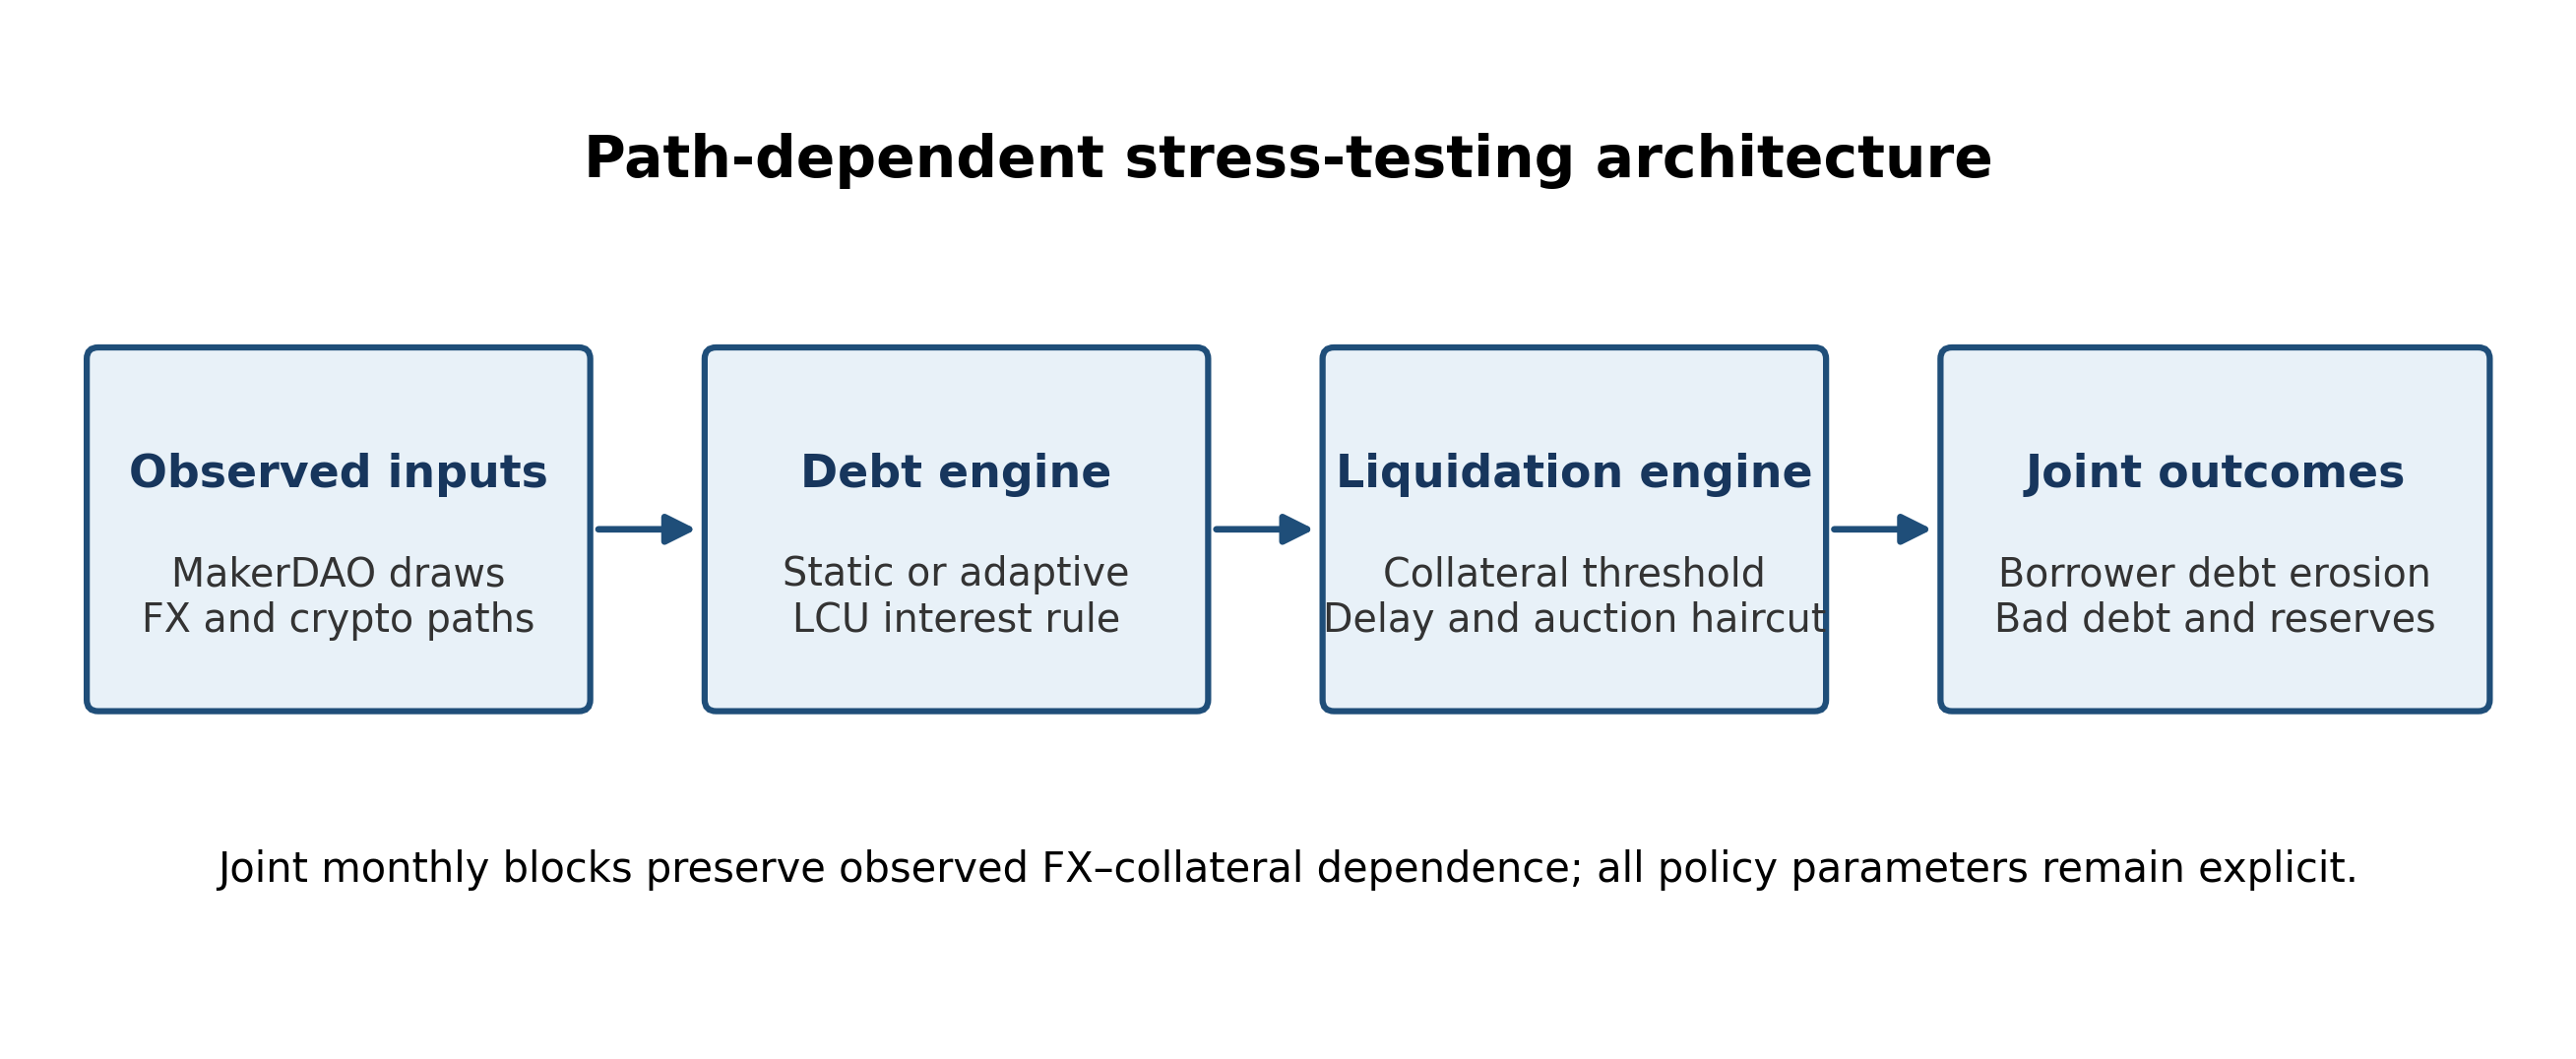
\includegraphics[width=0.96\textwidth]{figures/figure1_framework.png}
\caption{Path-dependent stress-testing architecture. Observed inputs determine joint paths; policy rules update debt; the liquidation engine maps threshold breaches into recoveries; borrower and protocol outcomes are reported from the same paths.}\label{fig:framework}
\end{figure*}

Let $E_t$ be LCU units per USD, so an increase is local-currency depreciation. Let $P_t$ be the USD collateral price, $D_t^{LCU}$ nominal debt, and $i_t$ the annual nominal borrowing rate applied during month $t$. For an initial USD-equivalent principal $D_0$, the USD debt factor is
\begin{equation}
 d_t \equiv \frac{D_t^{USD}}{D_0}
 = \frac{\prod_{m=1}^{t}(1+i_m/12)}{E_t/E_0}.
 \label{eq:debt}
\end{equation}
Currency depreciation lowers $d_t$; a higher rate raises it. If the initial collateral ratio is $c_0$, the collateral ratio at $t$ is
\begin{equation}
 CR_t = \frac{c_0(P_t/P_0)}{d_t}.
 \label{eq:cr}
\end{equation}
The first month with $CR_t<\theta$ is the breach month $\tau$. Execution occurs at $\tau+\delta$, where $\delta$ is the oracle/operational delay. If the breach is too late for execution inside the horizon, any actual collateral shortfall at maturity remains a protocol loss.

The auction recovery haircut responds to the fraction $L_t$ of portfolio exposure liquidated in the same month:
\begin{equation}
 h_t=\min\{0.30,\ h_0+\gamma L_t\}.
 \label{eq:haircut}
\end{equation}
For a position executed at $s$, bad debt per initial dollar is
\begin{equation}
 BD_s=\max\left\{d_s-c_0\frac{P_s}{P_0}(1-h_s),0\right\}.
 \label{eq:baddebt}
\end{equation}
Portfolio bad debt is the initial-collateral-weighted sum across positions. A reserve ratio $k$ is breached whenever $BD^{port}>k$. The tail capital statistic is $\CVaR_{0.99}$, the mean loss among outcomes at or above the 99th percentile. With a fixed USD reserve $R$, the CVaR-consistent debt ceiling is $R/\CVaR_{0.99}$.

The borrower metric is deliberately conservative. Surviving exposure receives terminal debt erosion $1-d_{12}$. Liquidated exposure receives no depreciation benefit and loses the collectible 13\% liquidation penalty, capped by collateral remaining after debt. The metric excludes collateral investment returns, taxes, conversion costs, and utility from borrowed funds; it is a financing-side diagnostic, not trading profit.

\section{Data and Reproducible Construction}\label{sec:data}

\subsection{MakerDAO activity and portfolio scale}

The on-chain calibration comes from the public MakerDAO Vat trace archive accompanying Chaleenutthawut et al. \cite{Chaleenutthawut2024}. The companion replication package decodes successful ETH-A \texttt{frob} calls with positive signed debt change using MakerDAO's documented accounting conventions \cite{MakerVatDocs,RokniLamouki2026}. The resulting sample contains 130,742 draws from 1 January 2020 through 31 July 2023, 16,846 unique \texttt{urn} identifiers, and DAI 13.318 billion in cumulative draw amount. An \texttt{urn} is an accounting position, not a verified person.

The draw distribution is highly skewed: the median is USD 4,791.78, the mean is USD 101,865.49, the 99th percentile is USD 1.046 million, and the maximum is USD 150.45 million. We publish 100 principal-quantile bins and the exact derivation code. The dynamic loss ratios do not require an assumption that all historical draws were simultaneously outstanding; the observed distribution is an empirical scale anchor, not an outstanding-debt estimate.

\subsection{FX and collateral prices}

Official monthly average exchange rates are obtained from OECD Main Economic Indicators through FRED: \texttt{ARGCCUSMA02STM} for ARS per USD and \texttt{CCUSMA02TRM618N} for TRY per USD \cite{FREDARS,FREDTRY}. ETH and BTC daily USD reference prices come from the free Coin Metrics Community Data archive, pinned to repository commit \texttt{f1a36afb962731c387bb03982758ab0103063da5} and aggregated to the last available daily observation in each month \cite{CoinMetricsData}. The shared sample comprises 43 level observations from January 2020 through July 2023 and 42 joint monthly returns.

\begin{figure*}[t]
\centering
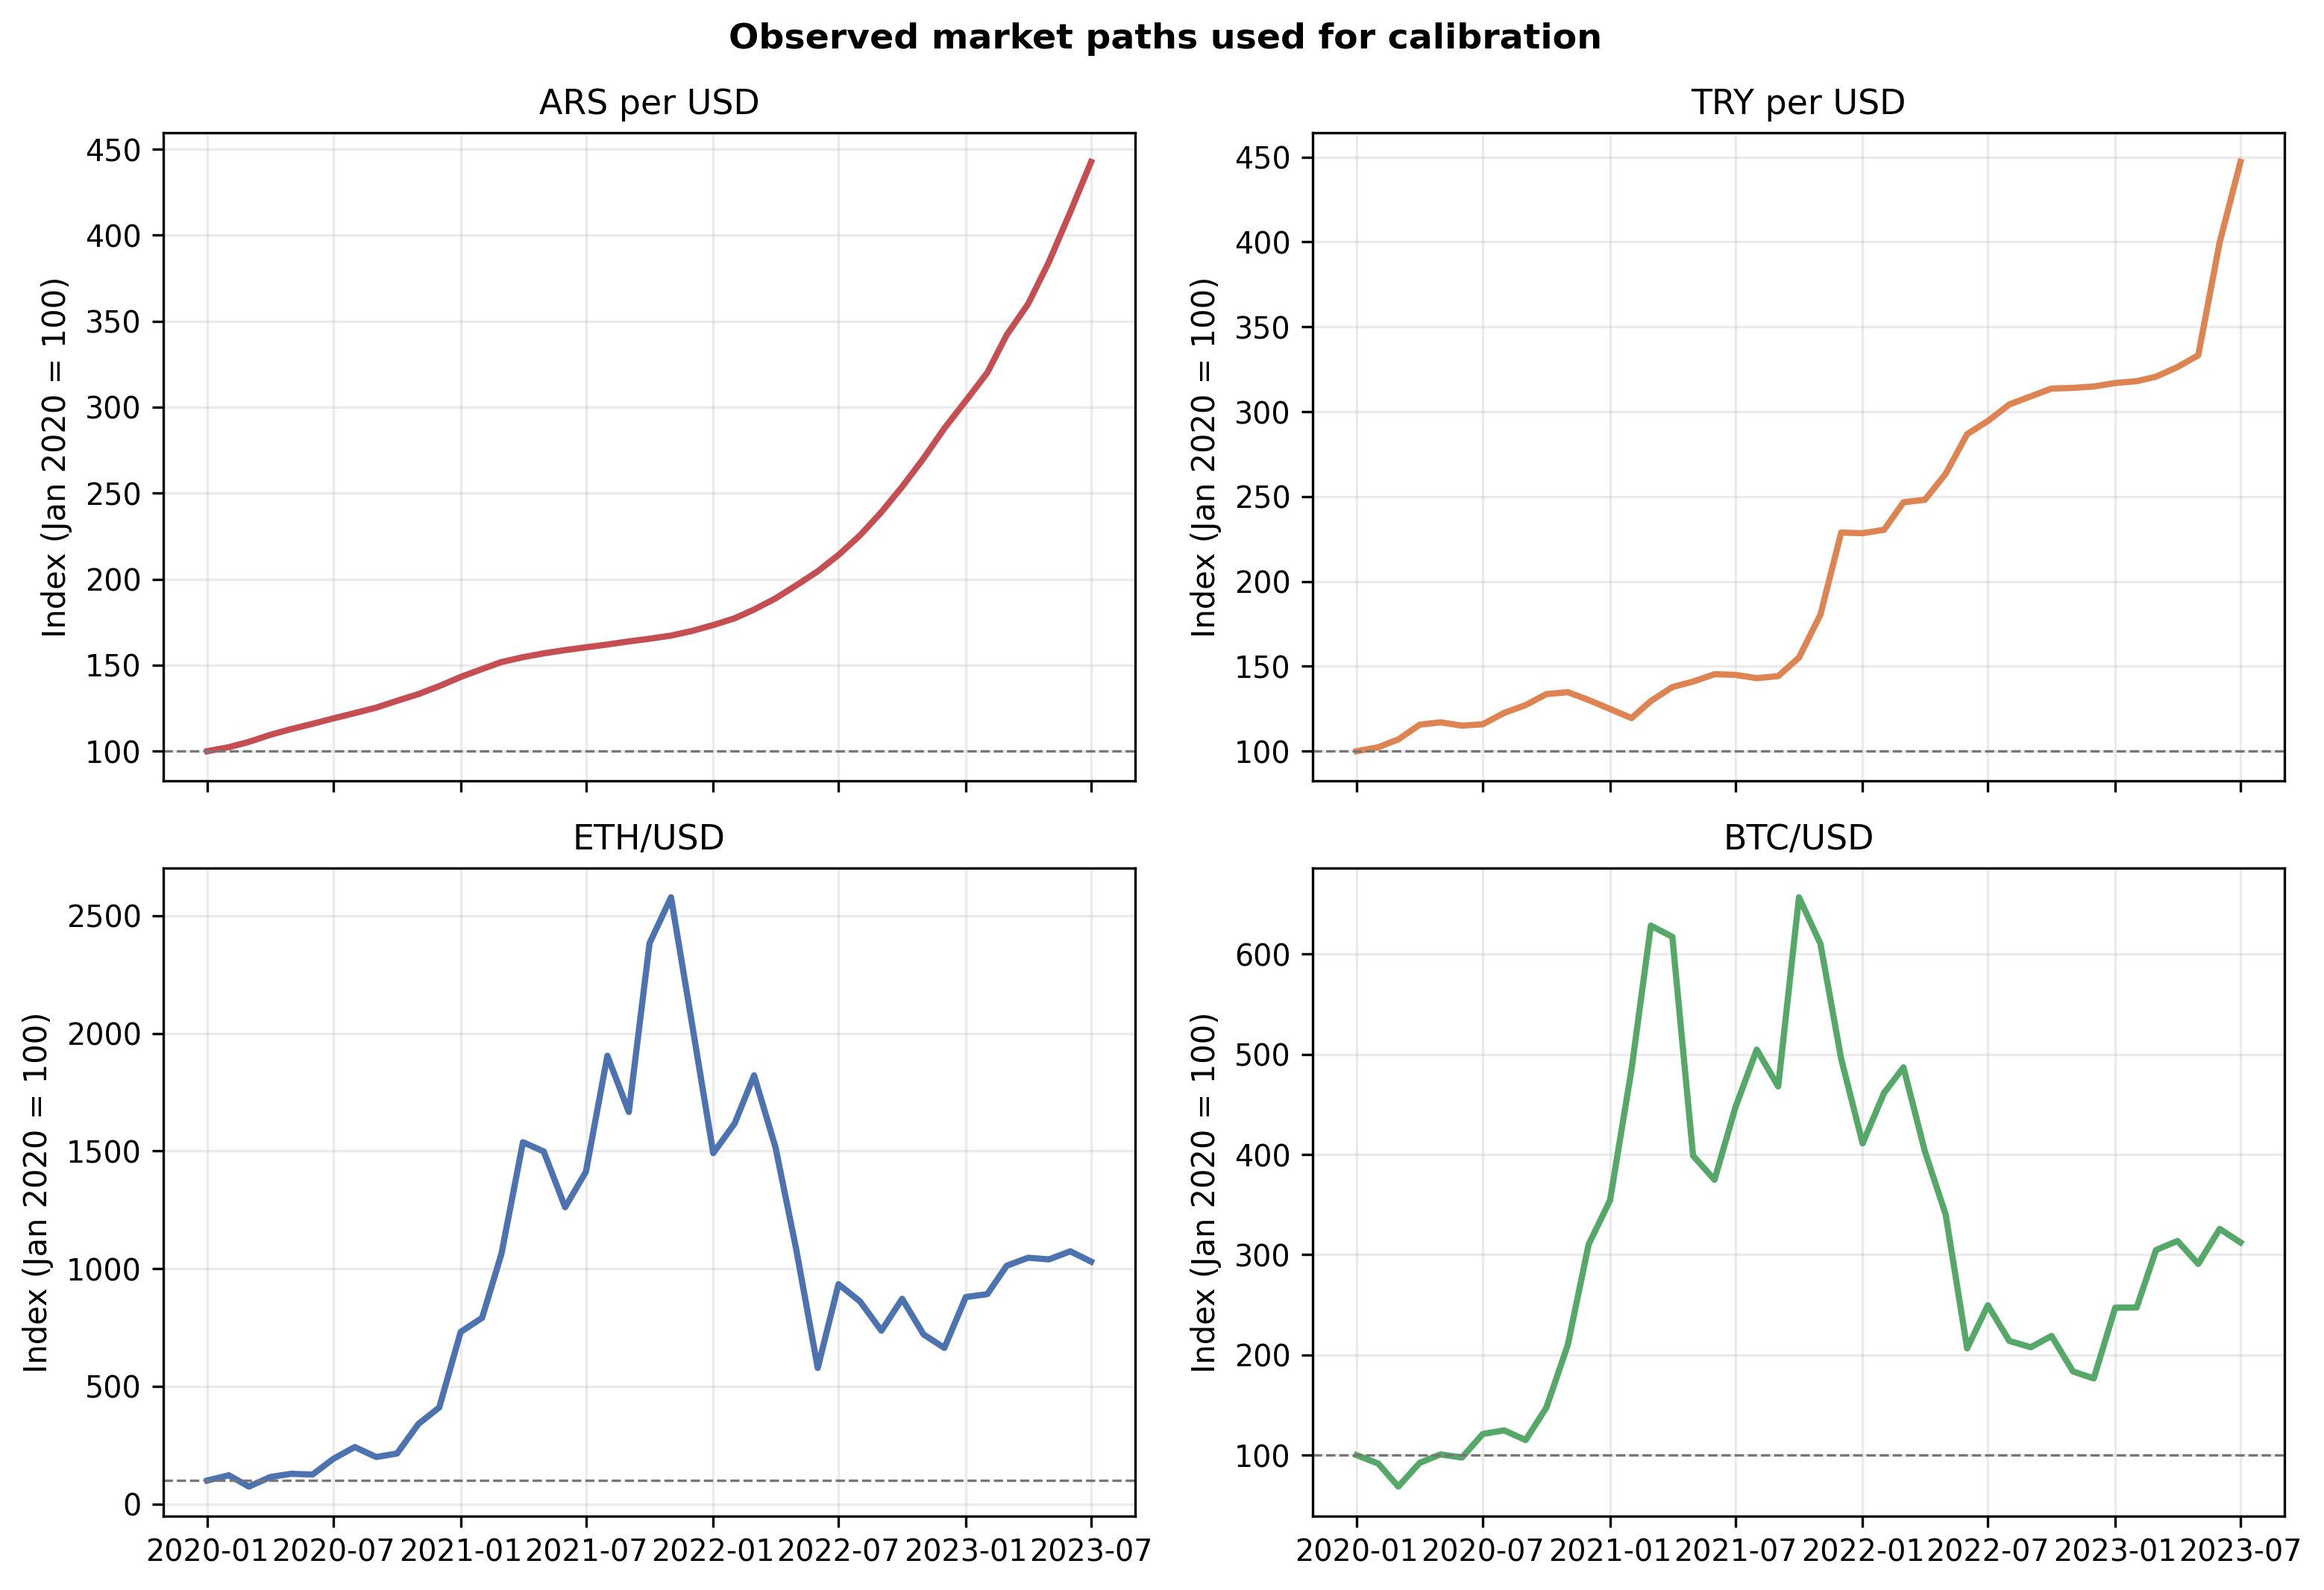
\includegraphics[width=0.93\textwidth]{figures/figure2_market_paths.png}
\caption{Observed market paths used for calibration. FX series are official monthly averages in LCU per USD; crypto series are Coin Metrics month-end reference prices. Each panel is indexed to January 2020.}\label{fig:paths}
\end{figure*}

\begin{figure*}[t]
\centering
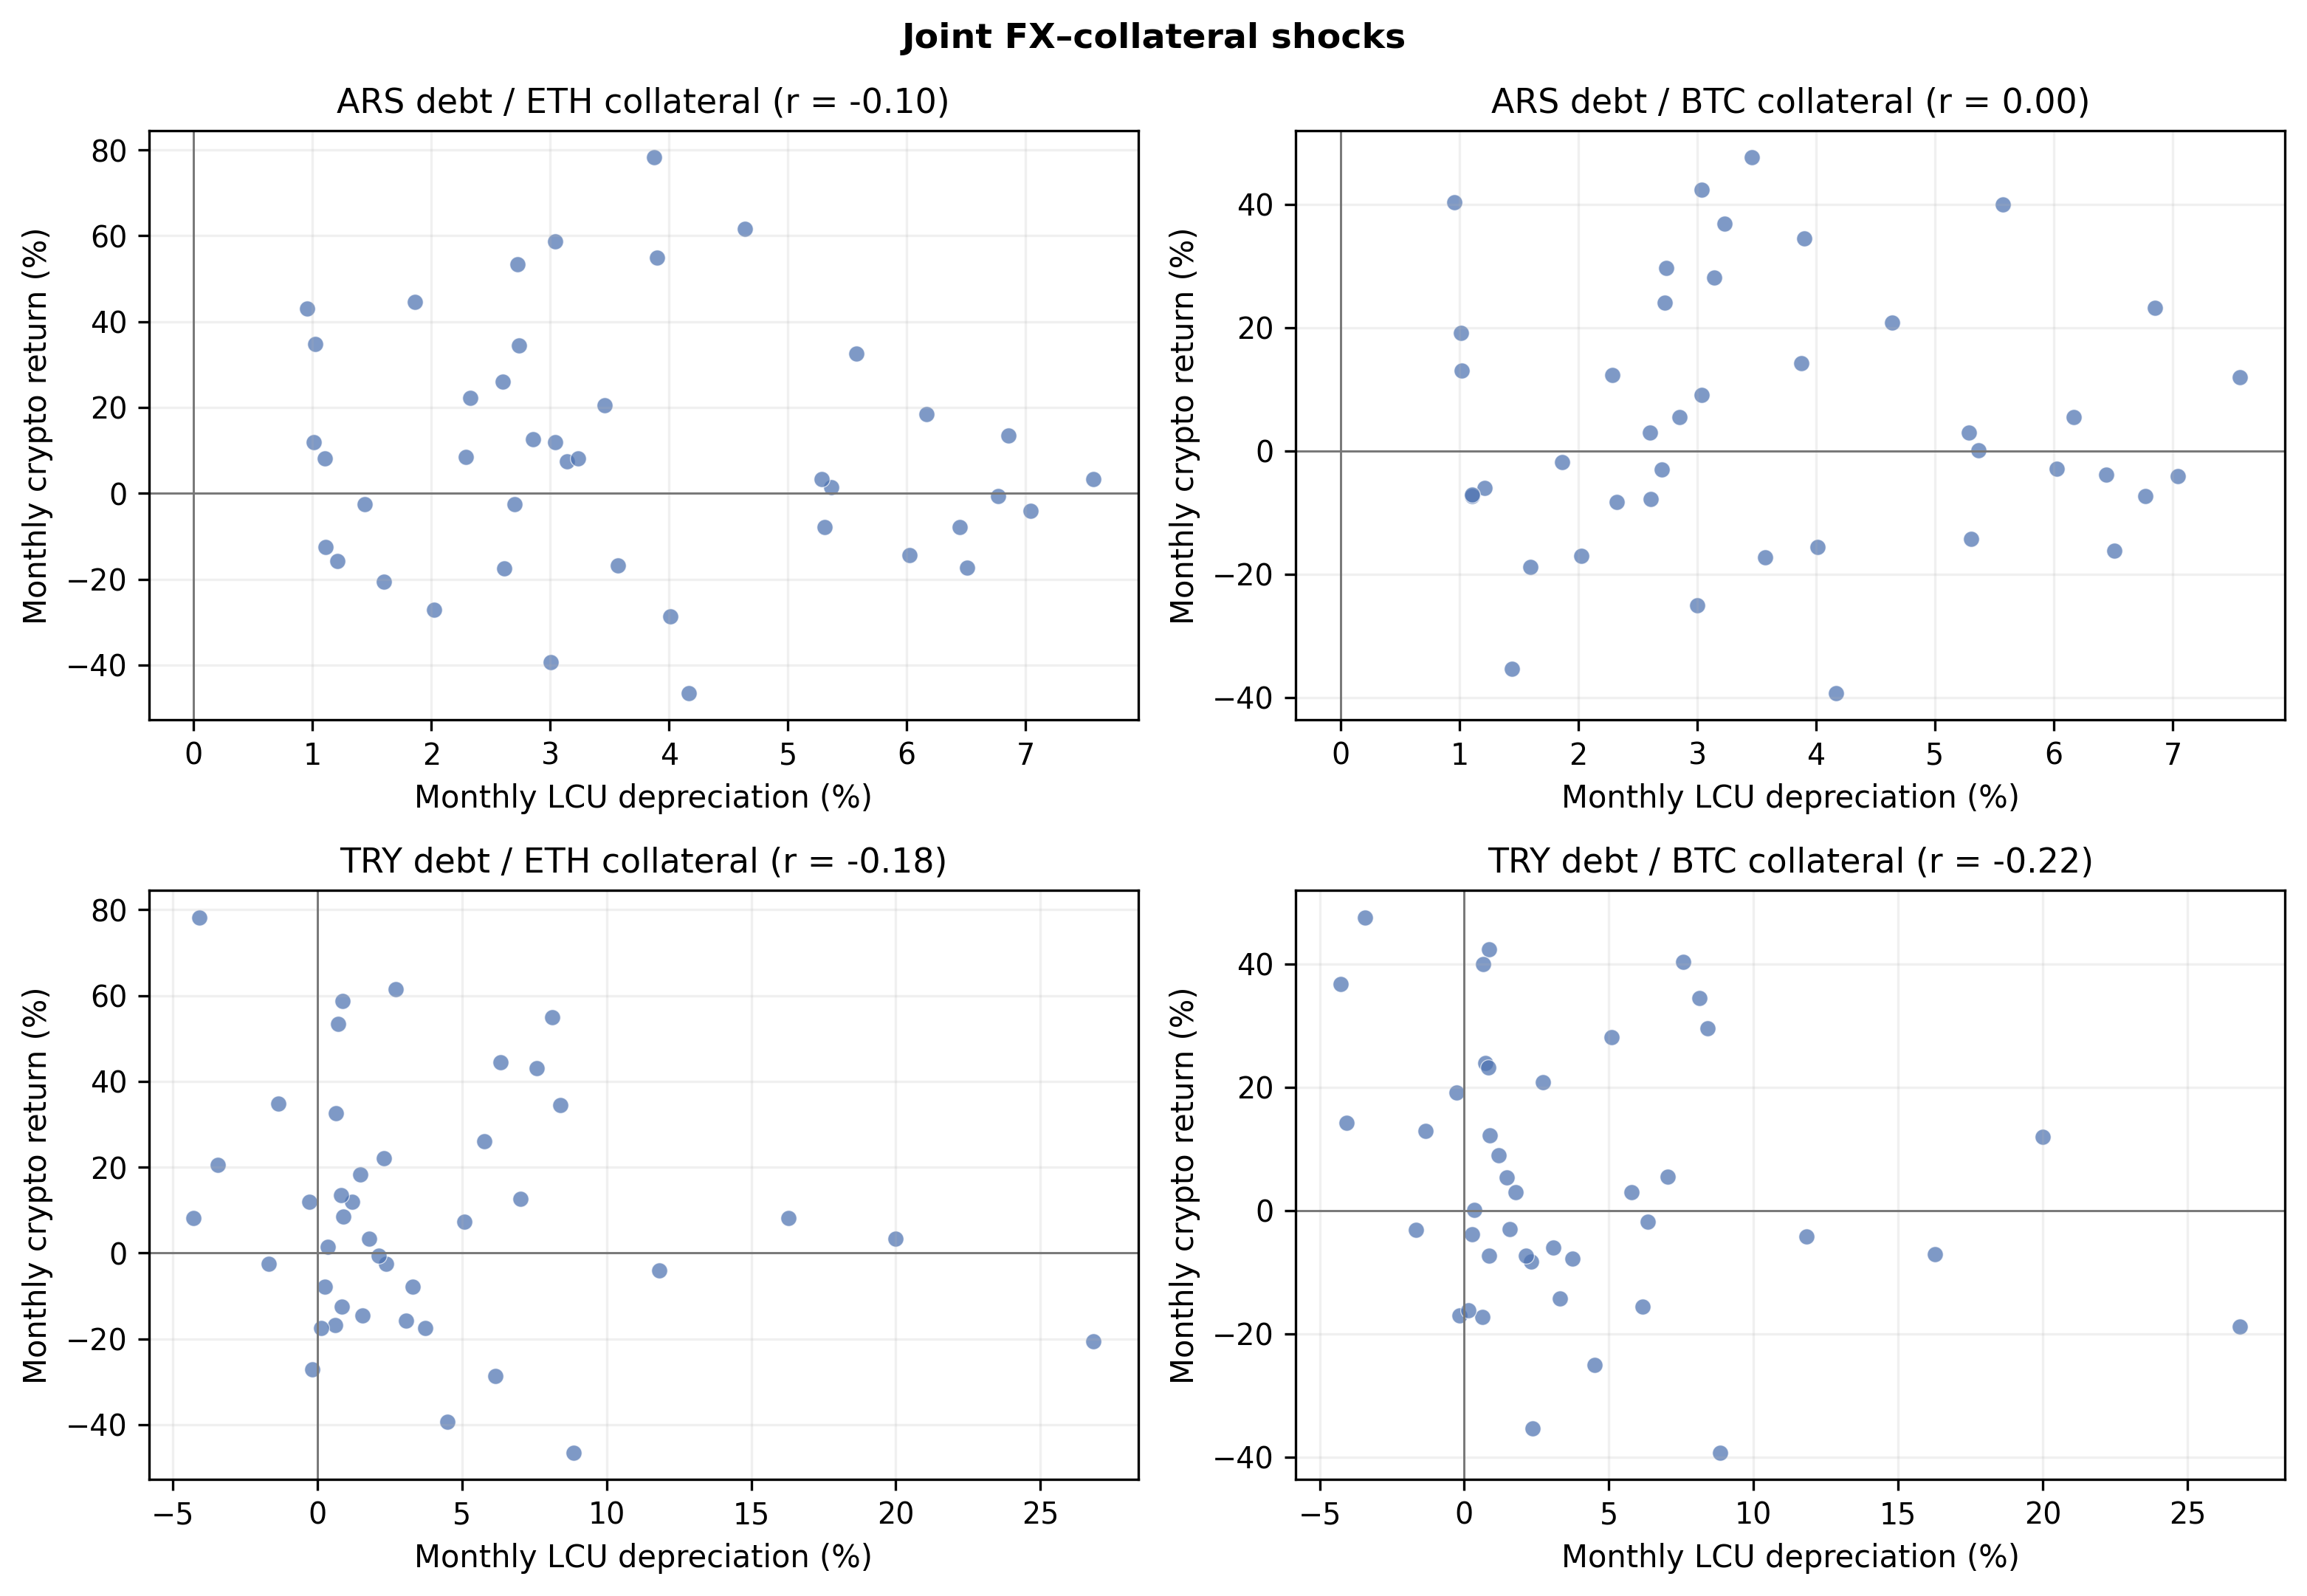
\includegraphics[width=0.93\textwidth]{figures/figure3_joint_shocks.png}
\caption{Joint monthly LCU depreciation and crypto returns. Upper-right observations combine depreciation with collateral appreciation; lower-right observations combine depreciation with collateral decline and are the main joint stress for a borrower.}\label{fig:joint}
\end{figure*}

\begin{table*}[t]
\centering
\caption{Data sources and construction.}\label{tab:data}
\small
\begin{tabularx}{\textwidth}{p{3.0cm}p{3.0cm}p{2.2cm}X}
\toprule
Input & Source & Coverage & Use \\
\midrule
MakerDAO debt draws & Public Vat trace archive and documented decoder \cite{Chaleenutthawut2024,MakerVatDocs} & 130,742 events, 2020-01 to 2023-07 & Portfolio scale and principal distribution \\
ARS/USD & OECD MEI via FRED, \texttt{ARGCCUSMA02STM} & 43 monthly levels & LCU debt translation \\
TRY/USD & OECD MEI via FRED, \texttt{CCUSMA02TRM618N} & 43 monthly levels & LCU debt translation \\
ETH/USD and BTC/USD & Coin Metrics Community Data & Daily, aggregated to 43 month-ends & Collateral paths \\
Joint returns & Authors' construction; no missing eligible months & 42 monthly pairs per currency--asset & Replay and moving-block bootstrap \\
\bottomrule
\end{tabularx}
\end{table*}

\begin{table*}[t]
\centering
\caption{Joint-return descriptives, February 2020--July 2023.}\label{tab:descriptive}
\small
\resizebox{0.92\textwidth}{!}{\begin{tabular}{llrrrr}
\toprule
Currency & Collateral & Months & FX mean (\%) & Crypto SD (\%) & Correlation \\
\midrule
ARS & ETH & 42 & 3.62 & 28.40 & -0.105 \\
ARS & BTC & 42 & 3.62 & 21.34 & 0.004 \\
TRY & ETH & 42 & 3.79 & 28.40 & -0.183 \\
TRY & BTC & 42 & 3.79 & 21.34 & -0.222 \\
\bottomrule
\end{tabular}
}
\begin{minipage}{0.95\textwidth}\footnotesize
\emph{Notes:} FX mean is the arithmetic mean monthly increase in LCU per USD. Crypto SD is the sample standard deviation of monthly USD returns. Correlation is contemporaneous Pearson correlation. There are 42 paired returns.
\end{minipage}
\end{table*}

Figure~\ref{fig:joint} illustrates why separate marginal shocks are insufficient. The contemporaneous correlations are modestly negative for ARS/ETH ($-0.105$), TRY/ETH ($-0.183$), and TRY/BTC ($-0.222$), but the sign alone does not identify liquidation risk. Joint adverse months---LCU depreciation and negative crypto return---occur in 35.71\% to 47.62\% of observations, depending on the pair. The block bootstrap therefore resamples paired, ordered observations rather than drawing FX and collateral independently.

\section{Stress-Test Design}\label{sec:method}

\subsection{Historical replay and moving-block bootstrap}

The historical replay applies the model to every contiguous 12-month window in the 42-return history, producing 31 realised paths per currency--collateral pair. The stochastic analysis uses the moving-block bootstrap of K\"unsch \cite{Kunsch1989}. A three-month starting index is selected uniformly with replacement; contiguous paired FX and crypto returns are copied until a 12-month path is formed. This preserves observed contemporaneous dependence and short-run clustering inside each block. We generate 20,000 paths per currency--collateral pair with seed \texttt{20260810}. Rate and mechanism comparisons within a pair use exactly the same paths.

The bootstrap is an empirical stress distribution, not a structural forecast. It assumes that the limited 2020--2023 return blocks are informative for scenario construction, and it cannot generate regimes absent from that history. Robustness tests use one- and six-month blocks.

\subsection{Rate rules}

Three nominal annual rate rules are compared:
\begin{enumerate}
  \item \textbf{Static 20\%:} $i_t=0.20$ in every month.
  \item \textbf{Adaptive 75\% pass-through:} $i_1=0.20$ and, thereafter,
  \begin{equation}
  i_t=\operatorname{clip}_{[0.05,1.50]}\left(0.10+0.75\widehat{\Delta E}_{t-1}^{ann}\right),
  \end{equation}
  where $\widehat{\Delta E}_{t-1}^{ann}$ is annualised geometric depreciation over up to the previous three months.
  \item \textbf{Indexed 100\% pass-through:}
  \begin{equation}
  i_t=\operatorname{clip}_{[0.05,2.00]}\left(0.05+\widehat{\Delta E}_{t-1}^{ann}\right).
  \end{equation}
\end{enumerate}
Both adaptive rules use only lagged information. They are design scenarios, not estimates of governance behaviour or optimal contracts.

\subsection{Collateral, liquidation, and reserves}

Initial collateral ratios lie on a 31-point grid from 150\% to 225\%. Exposure weights follow a triangular density with mode 175\%, chosen to place substantial mass near the liquidation boundary while retaining an upper buffer. This distribution is not observed from the trace archive and is therefore reported as an explicit stress assumption. The liquidation threshold is 150\%.

The timely mechanism executes in the breach month with an 8\% base auction haircut. The stressed mechanism executes one month later with a 15\% base haircut. Both add $0.20L_t$ for simultaneous liquidation, capped at a total haircut of 30\%. Reserve ratios are 5\%, 10\%, and 20\% of initial debt. Robustness varies the block length, base haircut, delay, congestion slope, and liquidation threshold one at a time.

\begin{table*}[t]
\centering
\caption{Baseline model parameters.}\label{tab:parameters}
\small
\begin{tabularx}{\textwidth}{p{4.0cm}p{3.0cm}X}
\toprule
Parameter & Baseline & Interpretation \\
\midrule
Horizon & 12 months & Common design and replay horizon \\
Bootstrap paths & 20,000 per pair & Three-month joint moving blocks; seed 20260810 \\
Initial collateral ratio & 150--225\%; mode 175\% & Triangular exposure distribution on 31 grid points \\
Liquidation threshold & 150\% & Breach trigger \\
Timely auction & 0-month delay; 8\% base haircut & Base execution design \\
Stressed auction & 1-month delay; 15\% base haircut & Operational stress design \\
Congestion surcharge & $0.20\times$ monthly liquidated share & Endogenous market-depth proxy; total haircut capped at 30\% \\
Borrower penalty & 13\% of debt, collateral-capped & Applied only to executed liquidations \\
Reserve ratios & 5\%, 10\%, 20\% & Protocol loss-absorption grid \\
Rate rules & Static 20\%; adaptive 75\%; indexed 100\% & Lagged pass-through to observed depreciation \\
\bottomrule
\end{tabularx}
\end{table*}

\subsection{Outcomes and validation}

For each path we retain: any-liquidation incidence, exposure-weighted liquidated share, mean bad debt, 99\% value-at-risk and CVaR, reserve-breach indicators, terminal debt erosion, survivor-weighted borrower benefit after penalty, and a CVaR-consistent debt ceiling for a USD 10 million reserve. Reported Monte Carlo confidence intervals use binomial standard errors for incidence and cross-path standard errors for mean loss. Every table value is machine-generated. The validation file checks path counts, row counts, finite outputs, and probability bounds.

\section{Results}\label{sec:results}

\subsection{Liquidation is path-dependent and widespread}

Figure~\ref{fig:liquidation} reports cohort-specific probabilities under timely execution. Lower initial collateral sharply increases liquidation, but rate policy also matters. A higher nominal rate increases $d_t$ and lowers $CR_t$ unless depreciation and collateral appreciation compensate. Consequently, the adaptive and indexed rules shift the liquidation curve upward relative to static 20\% pricing. This is the first element of the design trilemma: rate indexation removes the borrower subsidy by increasing the debt balance, but that same adjustment consumes collateral headroom.

\begin{figure*}[t]
\centering
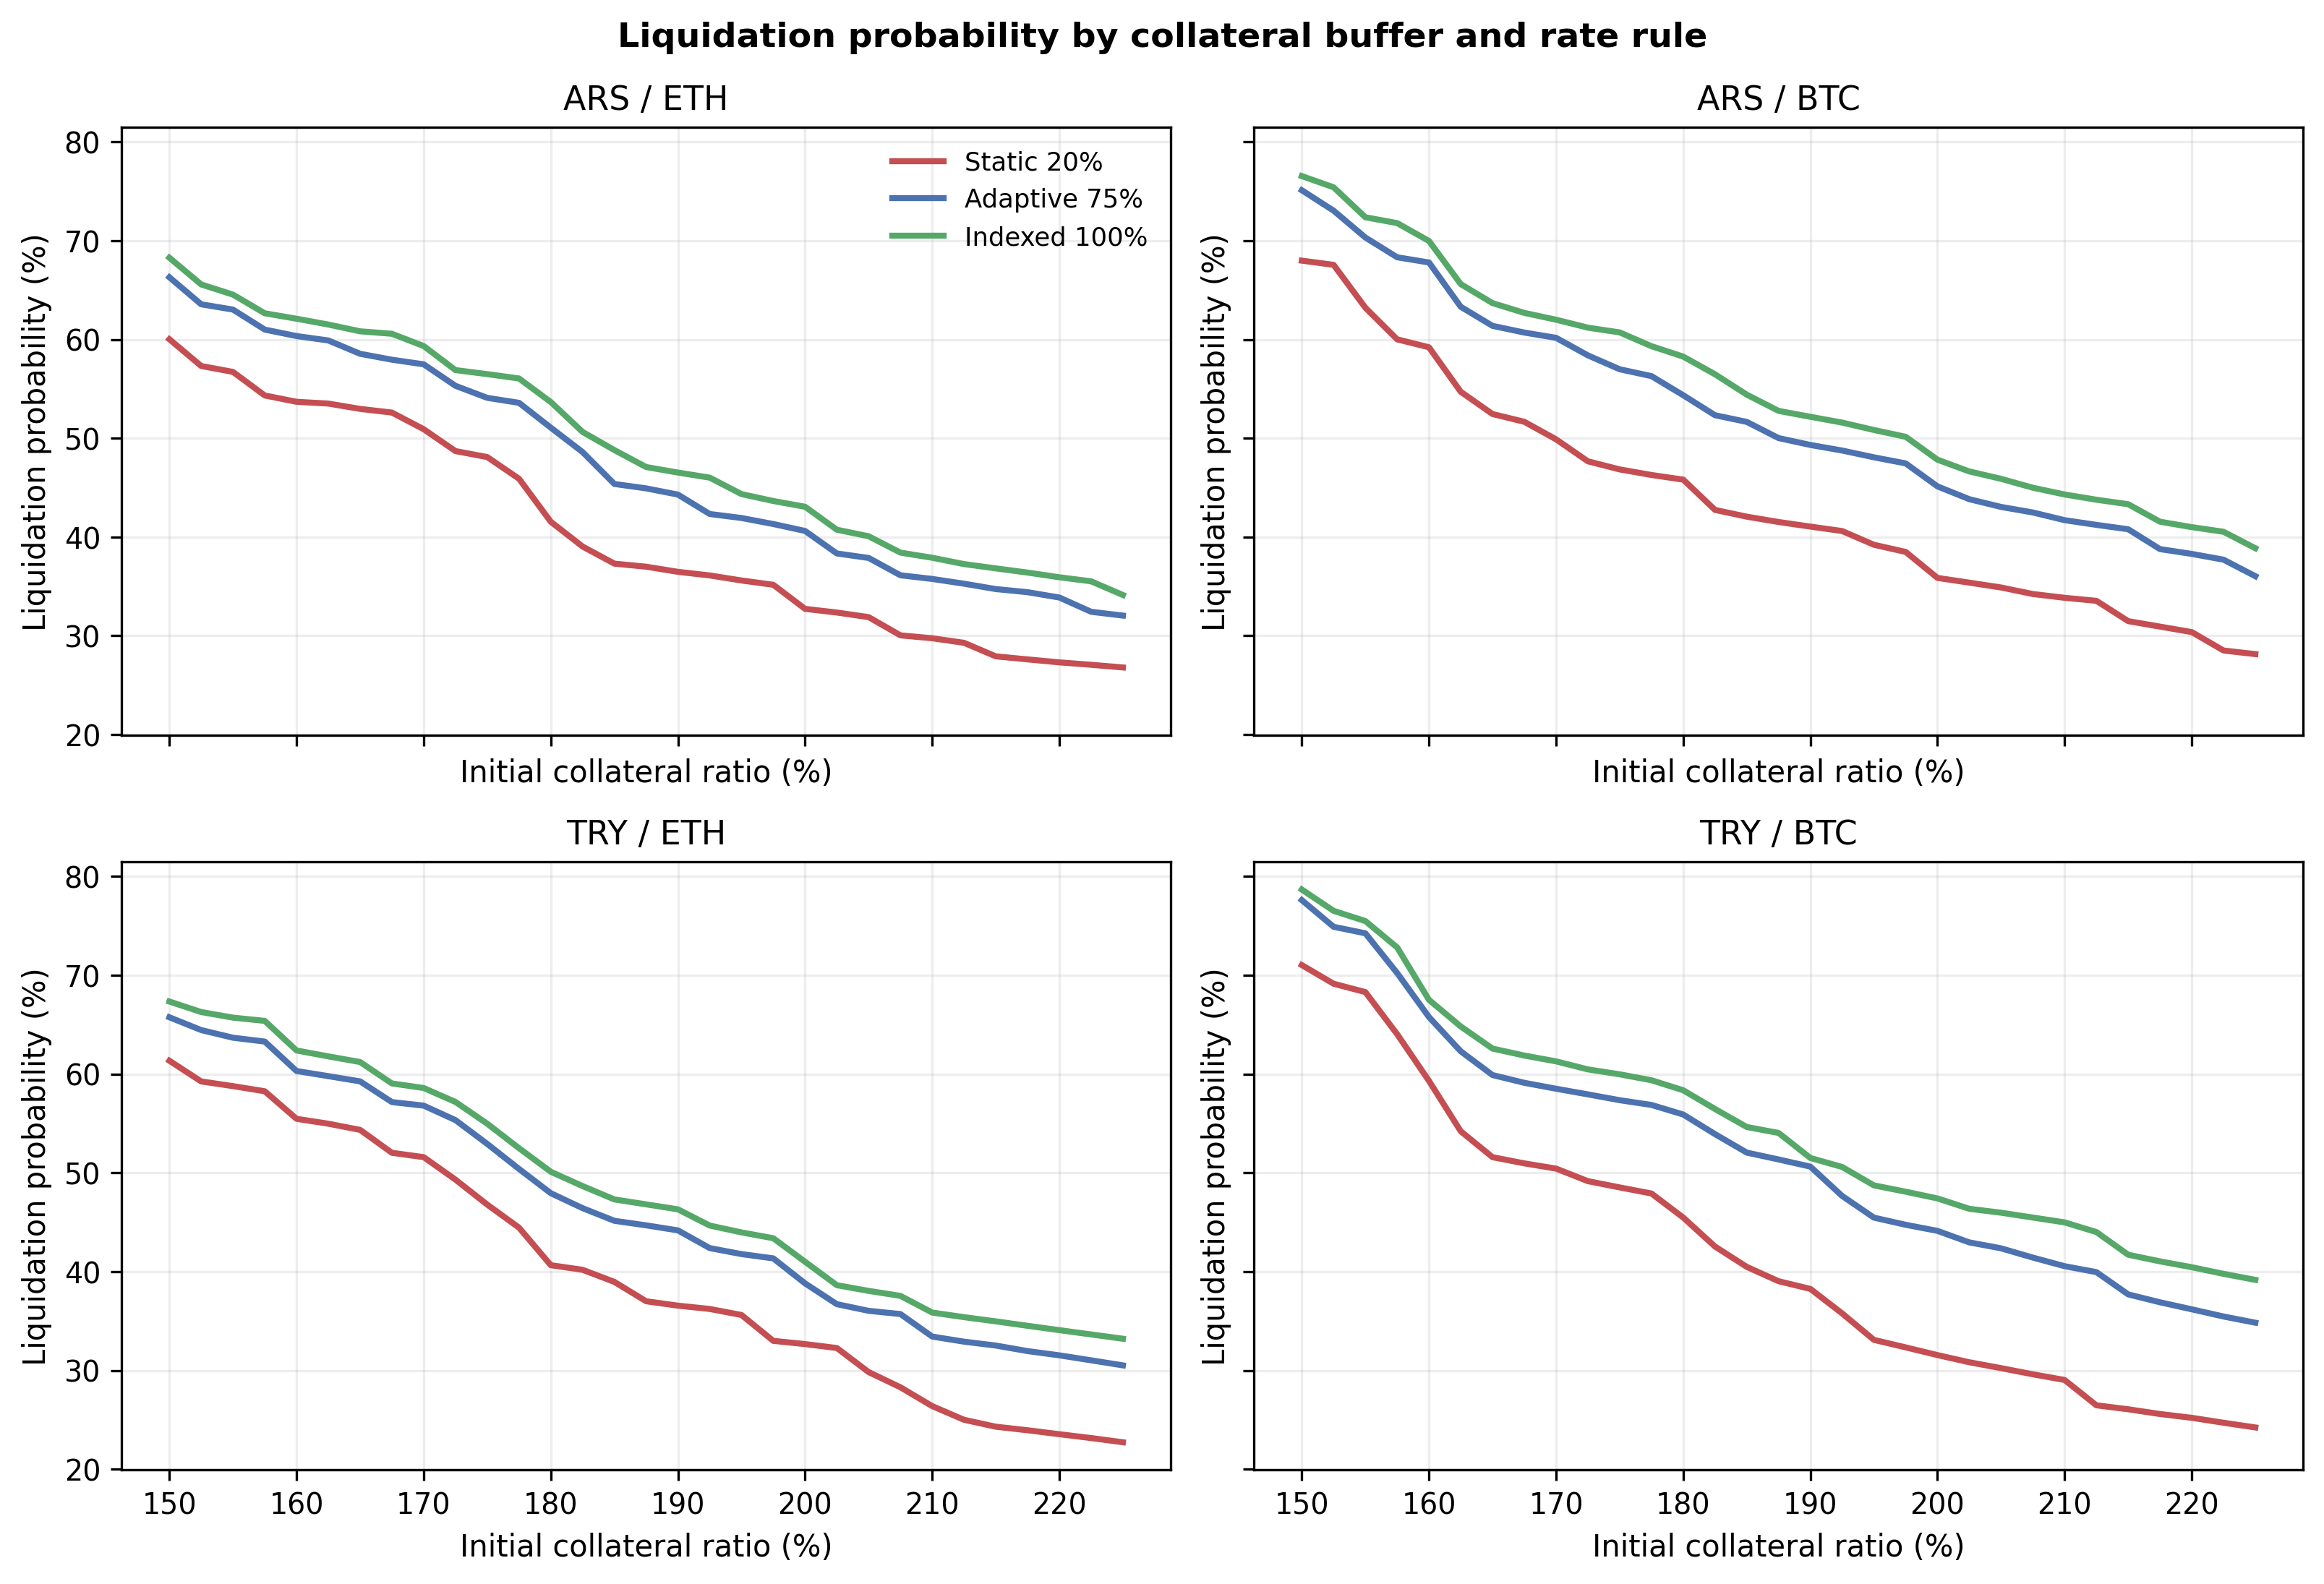
\includegraphics[width=0.94\textwidth]{figures/figure4_liquidation_curves.png}
\caption{Liquidation probability by initial collateral ratio and rate rule under timely execution. Each curve uses 20,000 joint paths and the same paths across rules within a currency--collateral pair.}\label{fig:liquidation}
\end{figure*}

Table~\ref{tab:main} focuses on ETH collateral and timely execution. Under static 20\% pricing, 41.91\% of ARS exposure and 41.71\% of TRY exposure is liquidated on average; borrower debt erosion remains positive because depreciation frequently exceeds nominal debt growth. Under the adaptive 75\% rule, liquidated exposure rises to 48.90\% and 47.96\%. Mean terminal debt erosion becomes negative: lagged rate increases more than offset the average USD debt reduction in the simulated paths. Indexed 100\% pricing intensifies this result.

\begin{table*}[t]
\centering
\caption{Main ETH-collateral outcomes under timely liquidation.}\label{tab:main}
\small
\resizebox{0.94\textwidth}{!}{\begin{tabular}{lllrrrr}
\toprule
Currency & Rate rule & Mechanism & Liquidated (\%) & Bad debt (\%) & CVaR$_{99}$ (\%) & Debt erosion (\%) \\
\midrule
ARS & Static 20\% & Timely & 41.91 & 2.77 & 27.04 & 19.31 \\
ARS & Adaptive 75\% & Timely & 48.90 & 3.44 & 30.26 & -5.44 \\
ARS & Indexed 100\% & Timely & 51.21 & 3.65 & 32.68 & -13.70 \\
TRY & Static 20\% & Timely & 41.71 & 2.33 & 22.93 & 16.17 \\
TRY & Adaptive 75\% & Timely & 47.96 & 3.21 & 25.75 & -8.01 \\
TRY & Indexed 100\% & Timely & 50.05 & 3.66 & 28.57 & -16.90 \\
\bottomrule
\end{tabular}
}
\begin{minipage}{0.97\textwidth}\footnotesize
\emph{Notes:} Liquidated is the expected exposure share executed during the 12-month horizon. Bad debt and CVaR are percentages of initial principal. Debt erosion is $1-d_{12}$ before conditioning on liquidation; negative values mean that nominal rates more than offset depreciation on average.
\end{minipage}
\end{table*}

\subsection{Borrower benefit and protocol loss form a frontier}

Figure~\ref{fig:frontier} places mean protocol bad debt against survivor-weighted borrower benefit. Static pricing lies above the zero-benefit line for both currencies but does not eliminate bad debt. The adaptive rules move downward and generally rightward: borrower benefit disappears while protocol loss increases because the higher debt balance triggers more collateral disposal and larger shortfalls during severe paths. This does not imply that permanently low rates are sustainable. It shows that rate policy alone cannot substitute for collateral buffers, auction capacity, or reserves.

Under static 20\% ETH pricing, the mean borrower financing-side benefit after modelled liquidation penalty is 6.78\% for ARS and 3.84\% for TRY. Under the adaptive 75\% rule it is $-8.28$\% and $-9.69$\%, respectively. These quantities deliberately set the benefit of liquidated exposure to zero before penalty and exclude gains or losses on the collateral asset; they should not be interpreted as realised user returns.

\begin{figure*}[t]
\centering
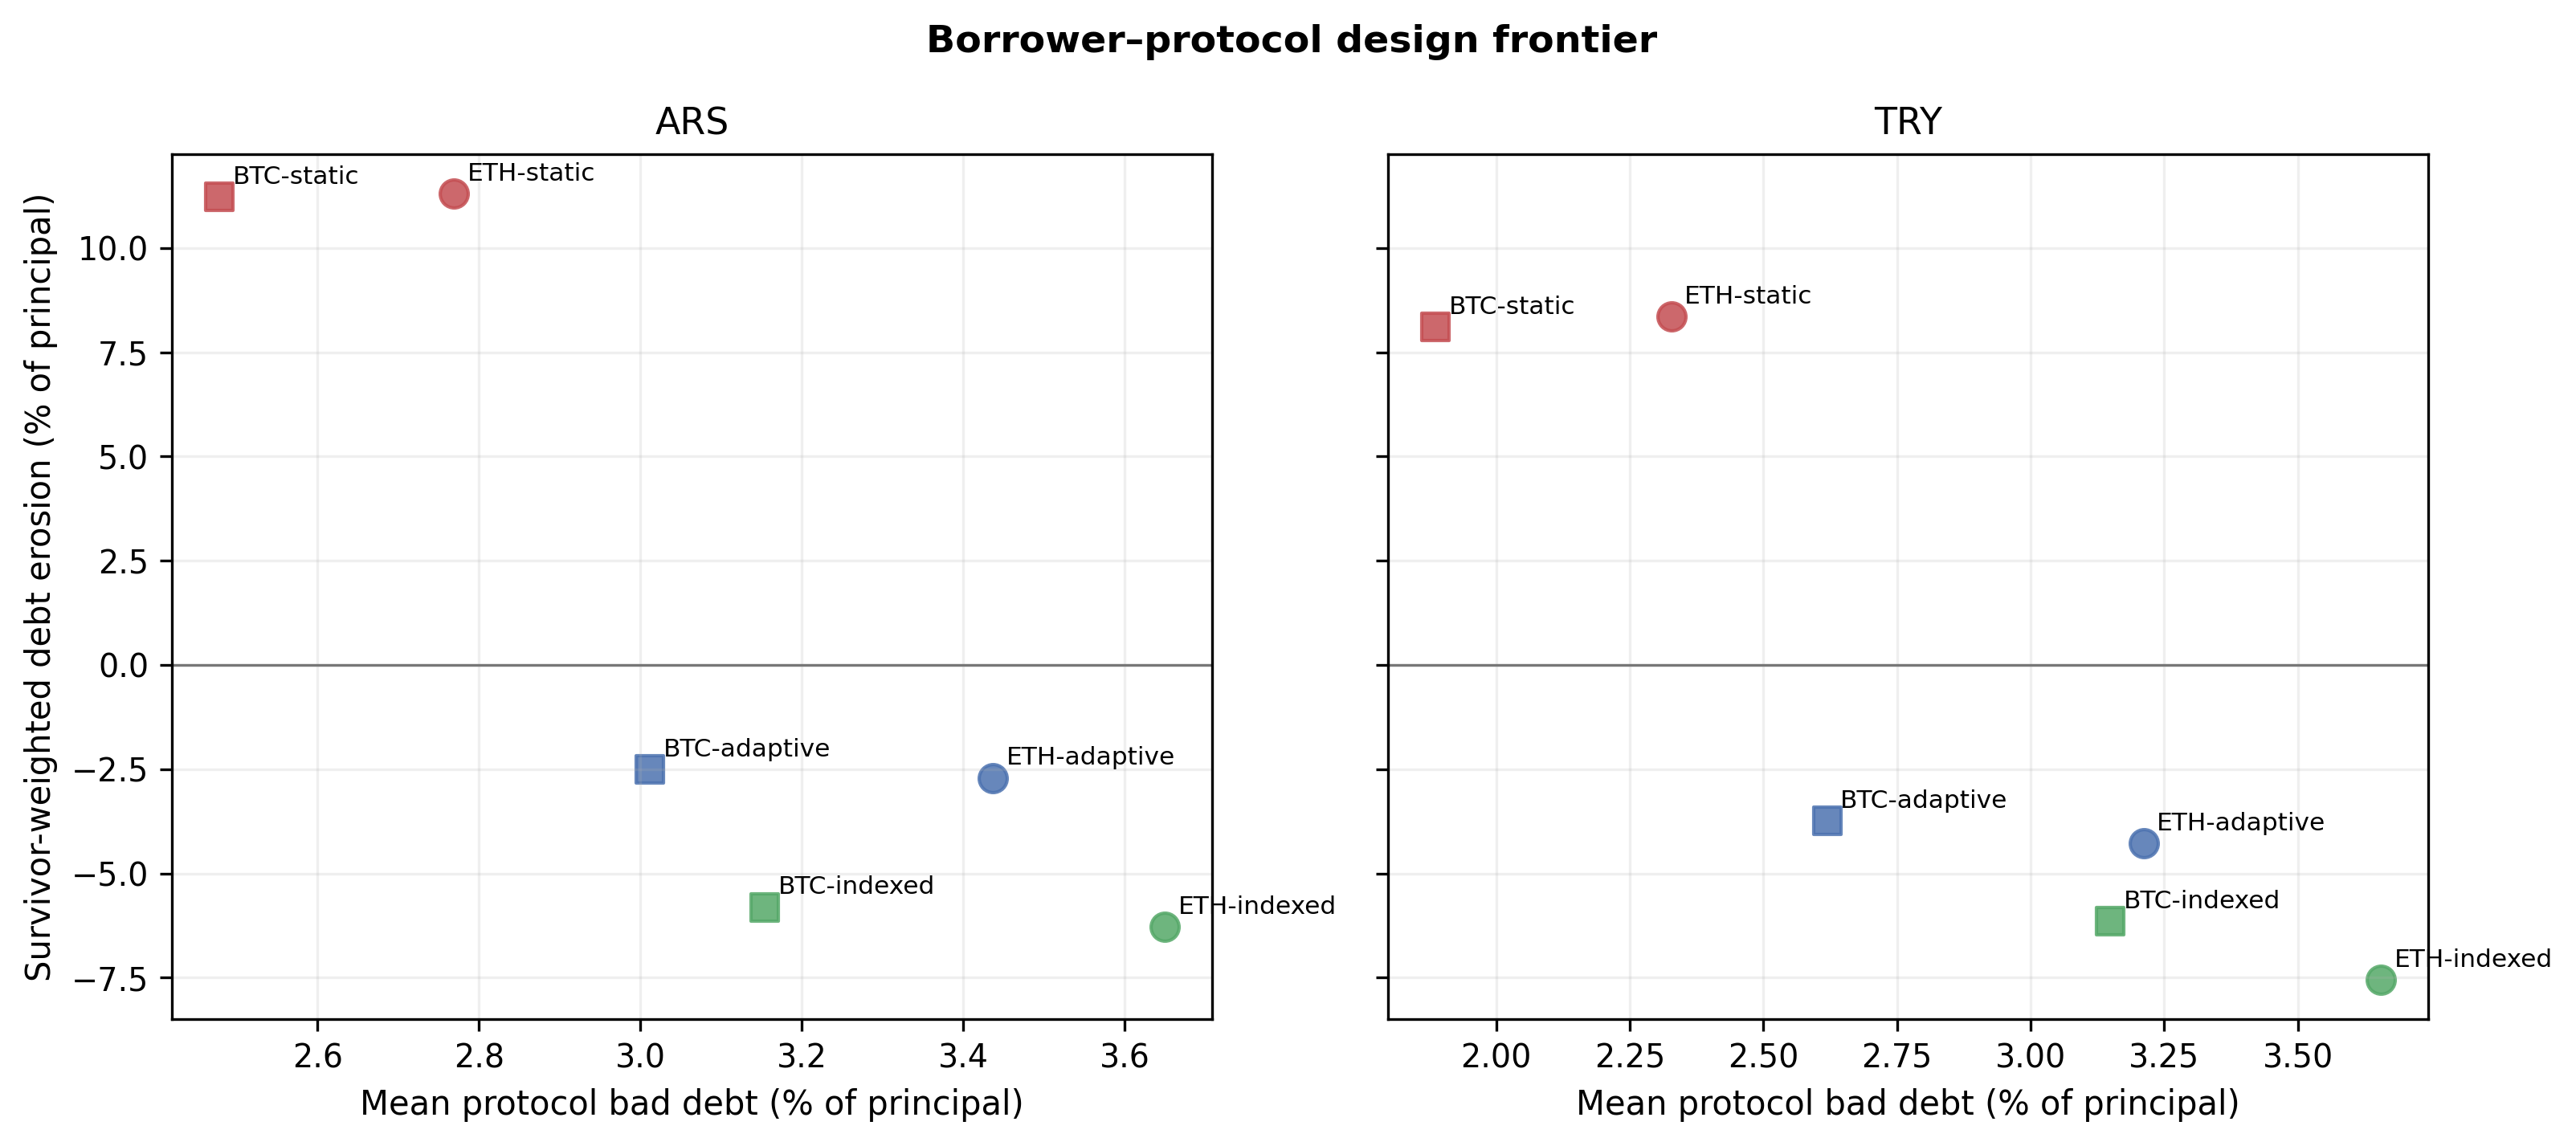
\includegraphics[width=0.92\textwidth]{figures/figure5_design_frontier.png}
\caption{Borrower--protocol design frontier under timely liquidation. Marker shape identifies collateral and colour identifies the rate rule. A desirable design would move upward and left, but no tested rule dominates on both dimensions.}\label{fig:frontier}
\end{figure*}

\subsection{Delay, auction stress, and reserve adequacy}

The execution mechanism materially changes loss even when the set of underlying return paths is fixed. Under adaptive ARS/ETH pricing, timely execution produces mean bad debt of 3.44\% and 99\% CVaR of 30.26\%. A one-month delay and 15\% base haircut raise these to 5.39\% and 52.51\%. TRY/ETH mean bad debt rises from 3.21\% to 4.76\%, while CVaR rises from 25.75\% to 46.63\%. The probability of exhausting a 10\% reserve rises from 10.97\% to 15.86\% for ARS and from 12.32\% to 15.03\% for TRY.

\begin{table*}[t]
\centering
\caption{Liquidation mechanism and reserve comparison under the adaptive 75\% rule with ETH collateral.}\label{tab:mechanism}
\small
\resizebox{0.96\textwidth}{!}{\begin{tabular}{lllrrrr}
\toprule
Currency & Mechanism & Any liquidation (\%) & Liquidated exposure (\%) & Bad debt (\%) & Reserve breach 10\% (\%) & Safe ceiling (USD m) \\
\midrule
ARS & Timely & 66.30 & 48.90 & 3.44 & 10.96 & 33.0 \\
ARS & One-month delay & 65.72 & 48.12 & 5.39 & 15.86 & 19.0 \\
TRY & Timely & 65.75 & 47.96 & 3.21 & 12.32 & 38.8 \\
TRY & One-month delay & 65.09 & 47.17 & 4.76 & 15.02 & 21.4 \\
\bottomrule
\end{tabular}
}
\begin{minipage}{0.97\textwidth}\footnotesize
\emph{Notes:} Any liquidation is the probability that at least one collateral-ratio cohort is executed; liquidated exposure is more informative for economic magnitude. The safe ceiling is $10$ million divided by 99\% CVaR and therefore assumes a USD reserve with no other claims.
\end{minipage}
\end{table*}

Figure~\ref{fig:reserve} shows that reserve adequacy is non-linear. Moving from a 5\% to 10\% reserve materially reduces breach probability, but tail outcomes remain; a 20\% reserve still breaches in 4.72\% of timely ARS paths and 4.05\% of timely TRY paths under the adaptive rule. Under delayed stress, the corresponding probabilities exceed 10\%. A reserve cannot be selected from mean loss alone.

\begin{figure*}[t]
\centering
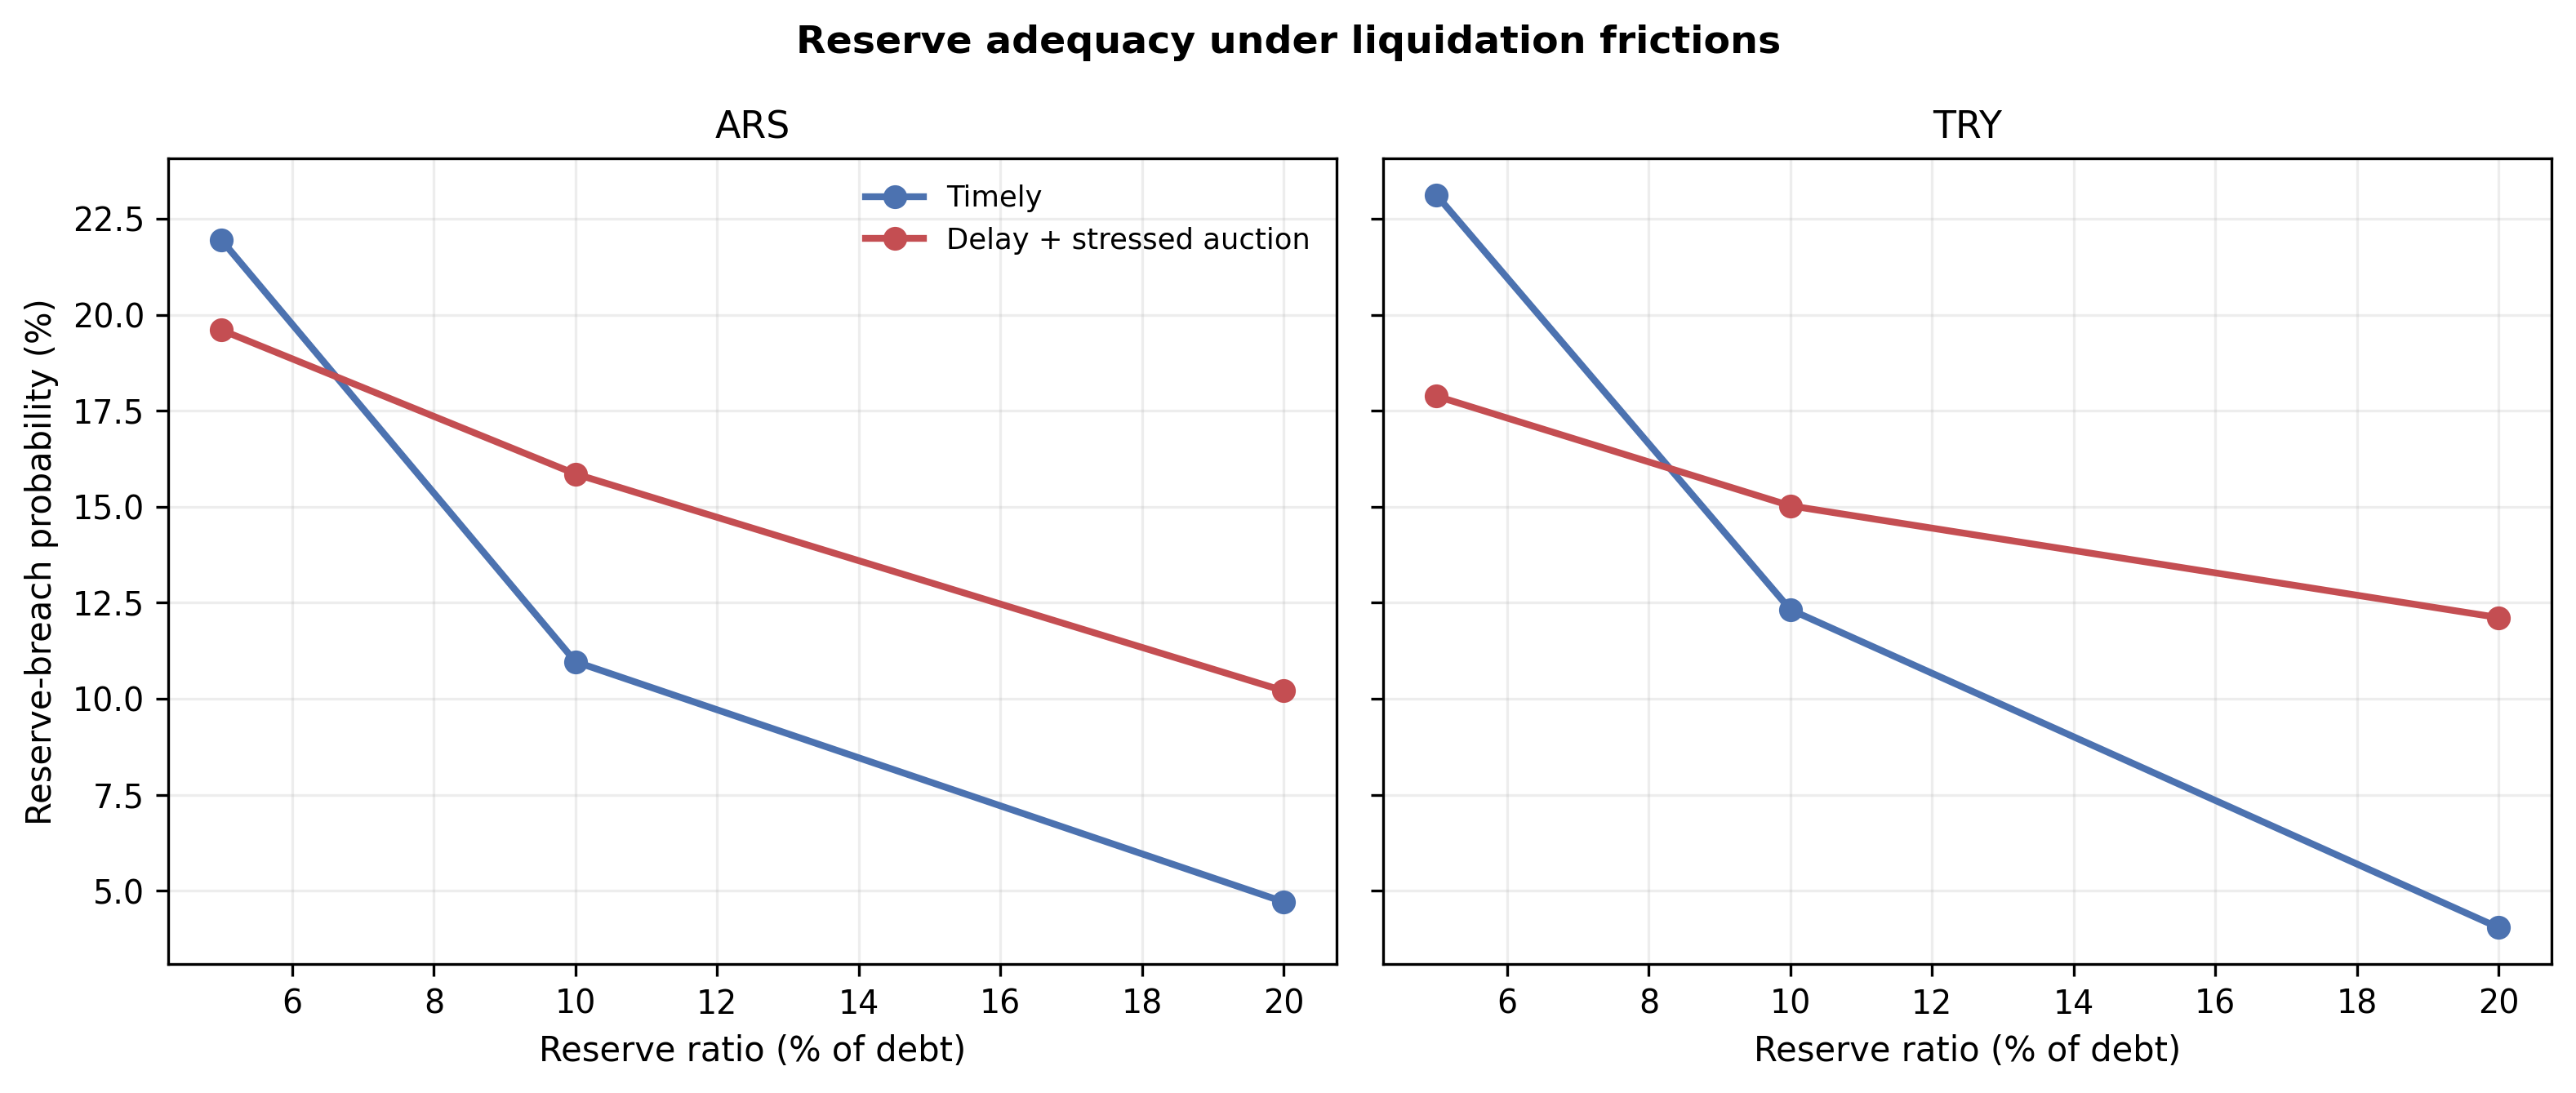
\includegraphics[width=0.90\textwidth]{figures/figure6_reserve_breach.png}
\caption{Reserve-breach probability for the adaptive 75\% rule with ETH collateral. The stressed line combines one-month execution delay with a 15\% base haircut.}\label{fig:reserve}
\end{figure*}

For a USD 10 million reserve, 99\% CVaR implies a debt ceiling of approximately USD 33.0 million for ARS/ETH and USD 38.8 million for TRY/ETH under timely adaptive execution. Under delayed stress, those ceilings fall to USD 19.0 million and USD 21.4 million. These are model-consistent capacity indicators, not recommended launch limits: peg liabilities, operating expenses, concentration, governance-token backstops, and legal claims are outside the calculation.

\subsection{Historical rolling-window replay}

The realised replay confirms that severe outcomes are not solely artifacts of random recombination. Across 31 windows under timely adaptive pricing, mean ETH liquidated exposure is 54.09\% for ARS and 53.82\% for TRY. Mean bad debt is 3.73\% and 3.96\%; the worst ETH windows begin in June 2022 and reach 27.00\% and 22.79\% bad debt. For BTC, the worst windows begin in July 2021.

\begin{table*}[t]
\centering
\caption{Realised 12-month rolling-window replay under adaptive 75\% pricing and timely liquidation.}\label{tab:replay}
\small
\resizebox{0.96\textwidth}{!}{\begin{tabular}{llrrrrl}
\toprule
Currency & Collateral & Mean liquidated (\%) & Maximum liquidated (\%) & Mean bad debt (\%) & Maximum bad debt (\%) & Worst start \\
\midrule
ARS & BTC & 59.25 & 100.00 & 3.63 & 20.49 & 2021-07 \\
ARS & ETH & 54.09 & 100.00 & 3.73 & 27.00 & 2022-06 \\
TRY & BTC & 60.42 & 100.00 & 3.47 & 18.34 & 2021-07 \\
TRY & ETH & 53.82 & 100.00 & 3.96 & 22.79 & 2022-06 \\
\bottomrule
\end{tabular}
}
\begin{minipage}{0.97\textwidth}\footnotesize
\emph{Notes:} Thirty-one overlapping windows are evaluated per pair. Maximum liquidated exposure can reach 100\% of the assumed initial-collateral distribution. Worst start identifies the window with maximum bad debt.
\end{minipage}
\end{table*}

\begin{figure*}[t]
\centering
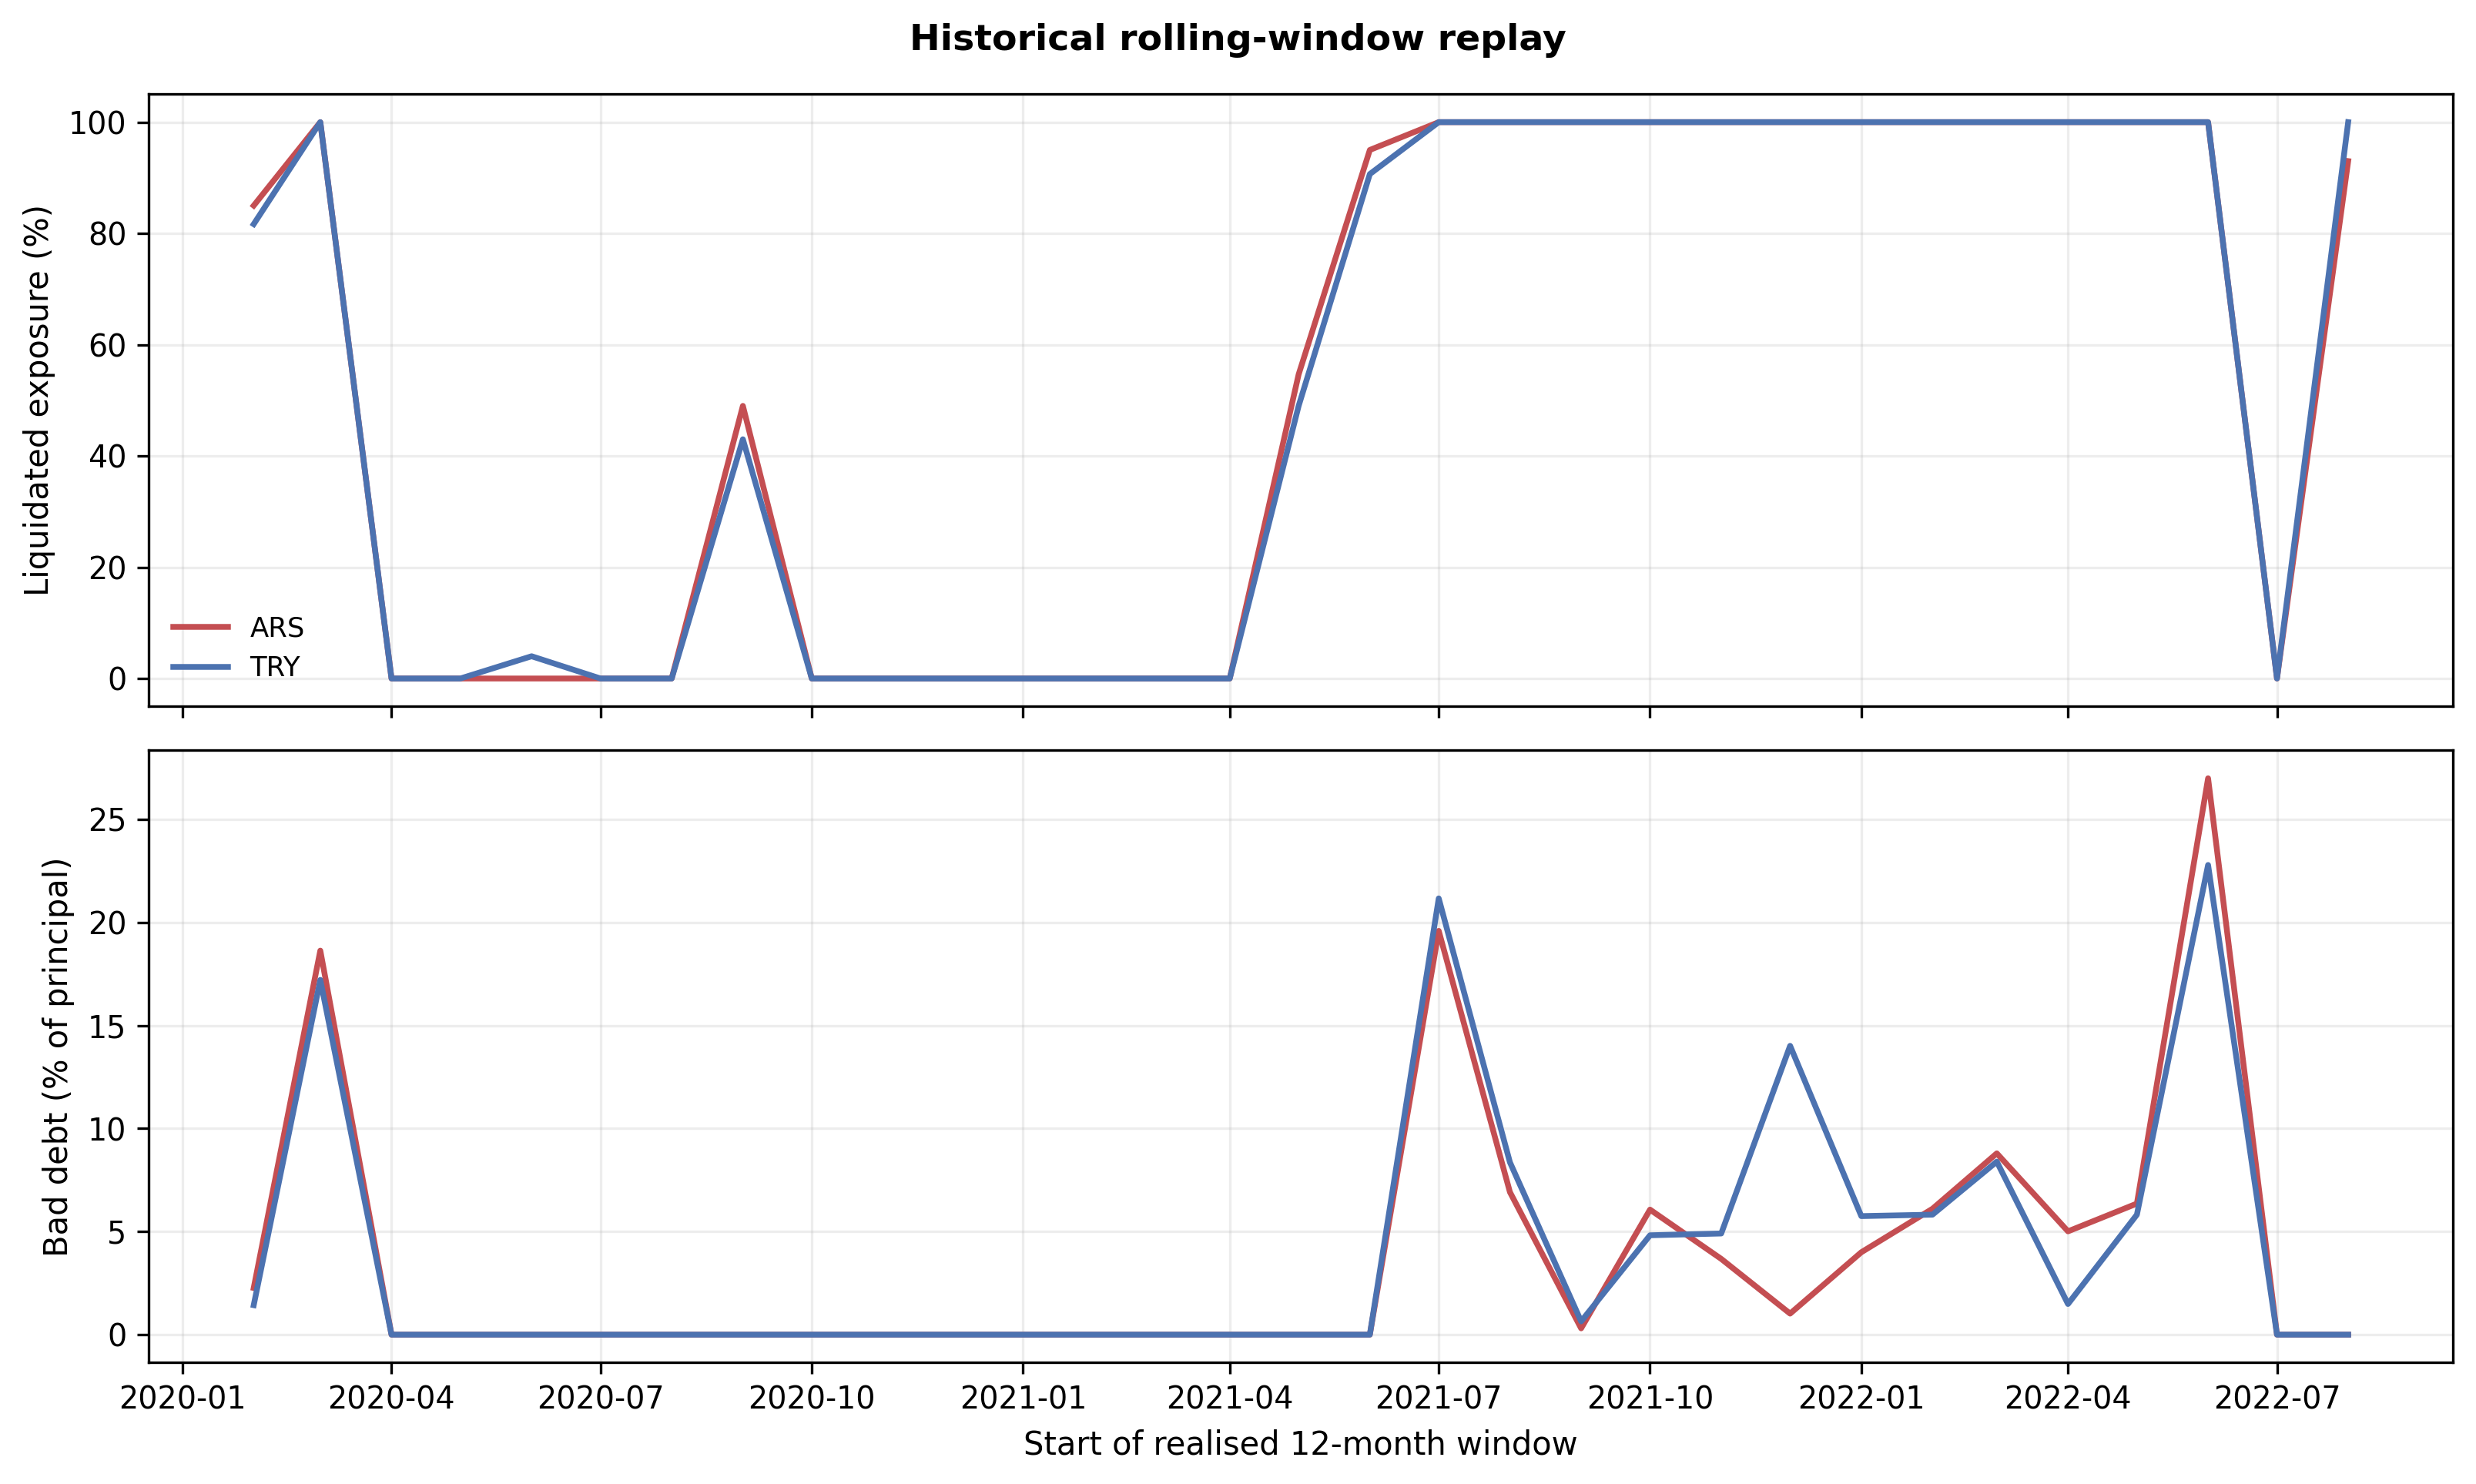
\includegraphics[width=0.93\textwidth]{figures/figure7_historical_replay.png}
\caption{Historical rolling-window replay for ETH collateral, adaptive 75\% pricing, and timely liquidation. Values are plotted by the first month of each realised 12-month window.}\label{fig:replay}
\end{figure*}

\section{Robustness and Sensitivity}\label{sec:robustness}

The robustness grid isolates one parameter at a time for ETH collateral and the adaptive 75\% rule. Changing the block length from one to six months leaves mean bad debt in a relatively narrow range. Auction and congestion assumptions matter more. For ARS, a 5\% base haircut produces mean bad debt near 2.7\%, while a 15\% haircut produces about 4.8\%. Setting the congestion slope to zero reduces mean bad debt to about 0.7\%. TRY shows the same ranking.

The liquidation threshold changes the timing and composition of sales. A lower 140\% threshold reduces liquidation frequency but permits deeper collateral deterioration before sale, increasing mean bad debt relative to a 160\% threshold in these paths. This illustrates why lower liquidation frequency is not synonymous with lower protocol loss.

\begin{table*}[t]
\centering
\caption{One-factor robustness for adaptive 75\% pricing with ETH collateral.}\label{tab:robustness}
\scriptsize
\resizebox{0.98\textwidth}{!}{\begin{tabular}{llrrrr}
\toprule
Currency & Variation & Value & Liquidated (\%) & Bad debt (\%) & CVaR$_{99}$ (\%) \\
\midrule
ARS & block length & 1 & 48.29 & 3.45 & 30.14 \\
ARS & block length & 3 & 49.01 & 3.48 & 30.47 \\
ARS & block length & 6 & 49.02 & 3.22 & 27.98 \\
ARS & auction haircut & 5\% & 49.01 & 2.71 & 27.67 \\
ARS & auction haircut & 15\% & 49.01 & 4.88 & 33.03 \\
ARS & oracle delay & 1 month & 48.19 & 4.65 & 50.32 \\
ARS & congestion slope & 0\% & 49.01 & 0.74 & 14.48 \\
ARS & liquidation threshold & 140\% & 42.83 & 4.79 & 35.41 \\
ARS & liquidation threshold & 160\% & 54.70 & 2.65 & 27.17 \\
TRY & block length & 1 & 49.11 & 3.05 & 26.56 \\
TRY & block length & 3 & 48.16 & 3.19 & 23.53 \\
TRY & block length & 6 & 48.70 & 3.07 & 23.59 \\
TRY & auction haircut & 5\% & 48.16 & 2.47 & 22.75 \\
TRY & auction haircut & 15\% & 48.16 & 4.39 & 28.17 \\
TRY & oracle delay & 1 month & 47.54 & 3.98 & 42.48 \\
TRY & congestion slope & 0\% & 48.16 & 0.56 & 10.57 \\
TRY & liquidation threshold & 140\% & 41.61 & 3.99 & 30.26 \\
TRY & liquidation threshold & 160\% & 54.14 & 2.58 & 22.90 \\
\bottomrule
\end{tabular}
}
\begin{minipage}{0.98\textwidth}\footnotesize
\emph{Notes:} Each currency uses 10,000 deterministic bootstrap paths per variation. Base-block mechanism variations reuse the same resampled paths. Parameter values are varied one at a time; rows are not alternative full designs.
\end{minipage}
\end{table*}

\begin{figure*}[t]
\centering
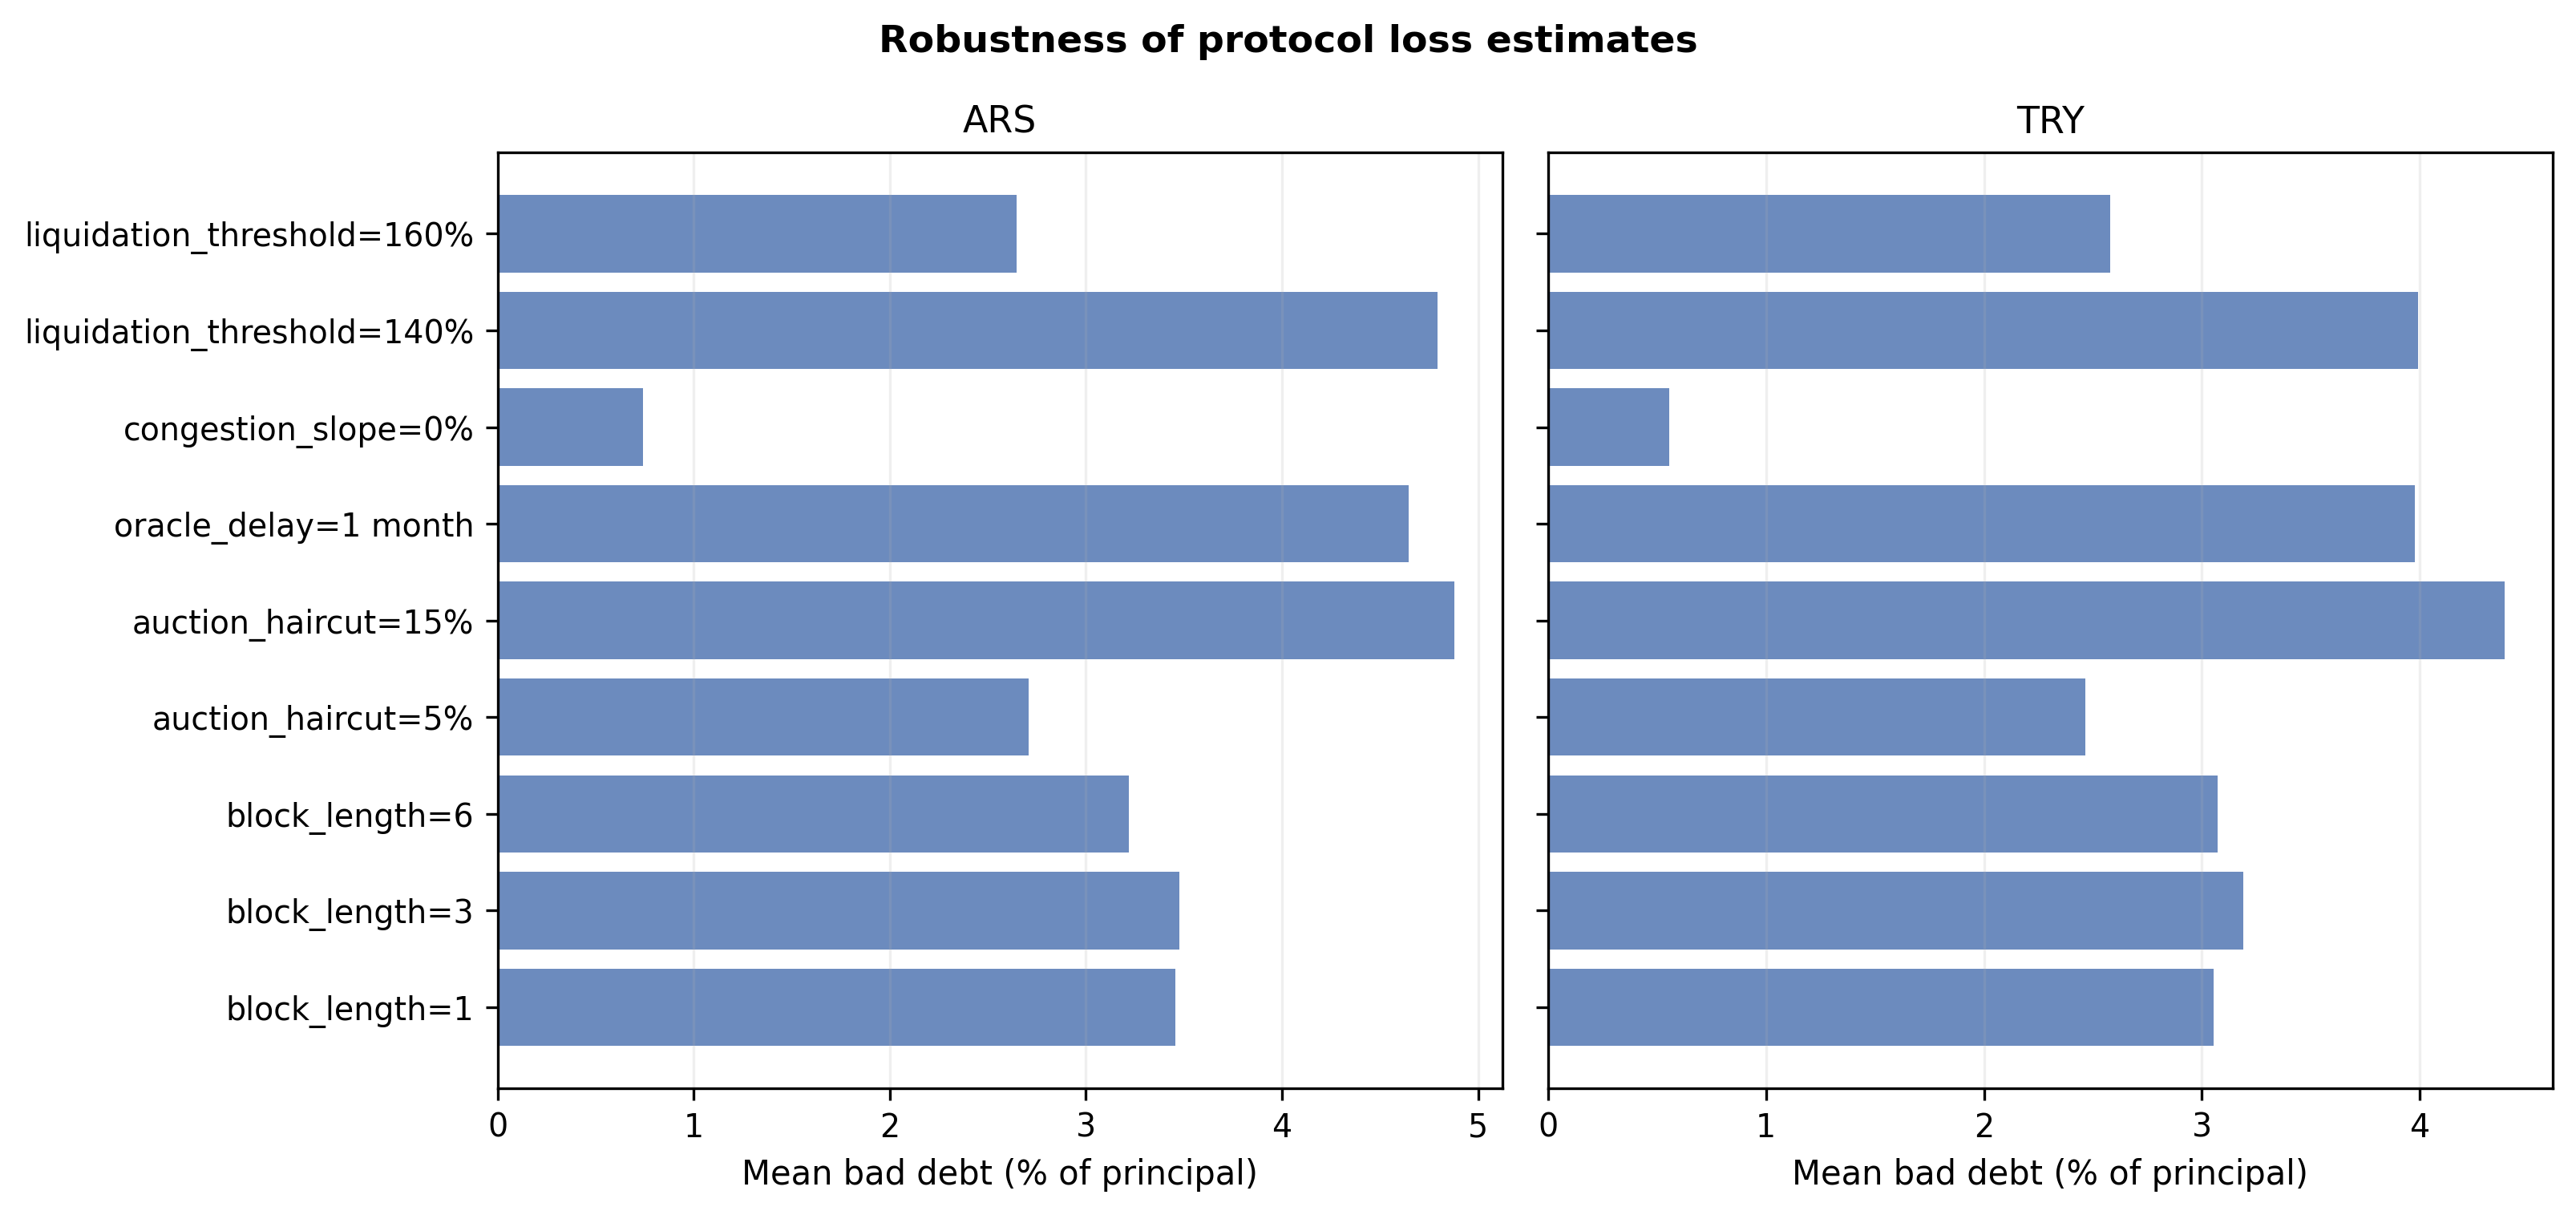
\includegraphics[width=0.91\textwidth]{figures/figure8_robustness.png}
\caption{Mean bad debt under robustness variations. Congestion and auction recovery are larger loss drivers than the bootstrap block length in the tested grid.}\label{fig:robustness}
\end{figure*}

Monte Carlo precision is high relative to the reported economic differences. For example, the 95\% interval for any liquidation under adaptive ARS/ETH pricing is 65.64--66.95\%, and the interval for mean bad debt is 3.34--3.53\%. These intervals measure simulation error conditional on the empirical return distribution and assumptions; they do not capture model uncertainty.

\section{Protocol-Design Implications}\label{sec:implications}

\subsection{A design trilemma}

The results reveal three competing objectives:
\begin{enumerate}
  \item preserve a material depreciation-driven financing advantage for borrowers;
  \item index borrowing rates strongly enough to prevent systematic erosion of the protocol's loan asset; and
  \item keep liquidation, auction loss, and reserve requirements low under volatile collateral.
\end{enumerate}
Within the tested architecture, no rate rule satisfies all three. Static pricing preserves the first objective but exposes the protocol to mispricing and demand expansion if depreciation accelerates. Full lagged indexation addresses the second only imperfectly and worsens the third by increasing debt after depreciation has already occurred. Safer designs require multiple controls rather than more aggressive rate feedback alone.

\subsection{Rates, buffers, and debt ceilings}

A practical rate rule should be forward-looking and state-contingent rather than a mechanical extrapolation of recent depreciation. It could combine expected inflation or forward-market information with utilisation, peg deviation, collateral volatility, and reserve adequacy. However, adding variables does not create executable FX liquidity. Governance should publish the formula, update cadence, data sources, caps, and emergency fallback.

Collateral policy should be currency- and asset-specific. A higher initial buffer lowers breach probability, while an excessively high liquidation threshold may increase sales during temporary shocks. Debt ceilings should be tied to tail loss and available reserves. Because the CVaR-consistent ceiling falls almost by half under delayed execution, operational readiness and auction depth are capital policy, not merely technical implementation details.

\subsection{Auction capacity and loss allocation}

The congestion result implies that liquidator and market-making capacity should be stress-tested before issuance grows. Measures may include diversified auction participants, bounded lot sizes, pre-committed backstop liquidity, circuit breakers, and transparent fallback rules. These mechanisms introduce their own governance and centralisation trade-offs. They should be evaluated under adverse conditions rather than inferred from normal-time spreads.

Residual loss allocation must also be explicit. Borrower collateral is first-loss protection, but bad debt can reach reserves, governance-token holders through recapitalisation, liquidity providers through impaired redemption, or stablecoin holders through a depeg. A protocol should not market borrower debt erosion without explaining which balance-sheet stakeholder funds it when asset recovery is insufficient.

\subsection{FX execution and peg credibility}

Official monthly FX rates provide an auditable numeraire but may differ from parallel or executable rates under capital controls. A live local-currency stablecoin requires mint and redemption channels, market makers with settlement access, and robust local legal analysis. Recent evidence that stablecoin flows interact with conventional FX markets reinforces the need to model market impact and parity deviations rather than treat an official reference rate as frictionless \cite{Aldasoro2026}.

\section{Limitations}\label{sec:limitations}

The study has ten material limitations. First, the system is counterfactual: no analysed MakerDAO borrower incurred ARS- or TRY-denominated debt. Second, historical MakerDAO draw timing and size need not represent demand for a local-currency product. Third, initial collateral ratios are an explicit triangular stress distribution because the source draw file does not provide a complete contemporaneous vault balance for every event. Fourth, 42 monthly joint returns are a small and unusual calibration window; block bootstrap paths cannot represent unobserved regimes. Fifth, monthly resolution cannot capture intramonth oracle latency, transaction ordering, MEV, or minute-level liquidation cascades. The one-month delay is therefore a coarse operational stress, not an estimate of real oracle delay.

Sixth, the haircut-congestion function is transparent but illustrative; it is not estimated from ARS- or TRY-stablecoin auctions. Seventh, official FX averages may not be executable and can differ materially from parallel markets. Eighth, the borrower metric excludes collateral opportunity cost, taxes, conversion spreads, stablecoin depeg, and the utility of borrowed funds. Ninth, the solvency calculation focuses on collateral recovery and a USD reserve; it does not model redemption runs, duration mismatch, governance-token dilution, or legal seniority. Tenth, overlapping historical windows are descriptive and not independent observations.

These limitations preclude claims of optimal pricing, live-protocol safety, or user profitability. They do not invalidate the comparative result that rate rules, collateral paths, liquidation frictions, and reserve policy must be evaluated jointly.

\section{Conclusion}\label{sec:conclusion}

This paper extends borrower-side debt erosion into a path-dependent protocol solvency problem. Using public MakerDAO draw calibration, official ARS and TRY exchange rates, Coin Metrics ETH and BTC prices, realised rolling windows, and 20,000 joint bootstrap paths, it finds that crypto-collateral liquidation remains material even when local-currency depreciation reduces the USD value of debt. Under adaptive 75\% pricing and timely ETH liquidation, roughly 48--49\% of the assumed exposure distribution is liquidated on average and mean bad debt is 3.2--3.4\% of principal. Delay and stressed auction recovery raise both mean and tail loss substantially.

Rate indexation is not a standalone cure. It removes the depreciation-driven borrower advantage but can increase liquidation by raising debt faster than collateral buffers adjust. Auction congestion, reserve capital, and debt ceilings therefore belong in the core product design. The central conclusion is conditional but clear: a local-currency DeFi lender may offer useful programmable credit, yet it cannot promise both persistent debt erosion and low protocol risk without identifying who supplies the missing value and how losses are absorbed. A live pilot would require higher-frequency executable FX data, observed user demand, audited contracts, market-maker commitments, legal review, and pre-funded loss capacity beyond this design study.

\section*{Data Availability}

The complete replication package is publicly available at \url{https://github.com/nikorokni/local-currency-defi-solvency-stress-test}. It includes the official FRED CSV files, pinned Coin Metrics analysis-window extracts, processed joint monthly panel, MakerDAO sample-construction and principal-calibration files, all result CSVs, machine-generated LaTeX tables, figures, source checksums, and validation anchors. The underlying MakerDAO event archive and its decoded event-level file are documented and linked to the companion repository because the raw archive is too large for ordinary Git hosting. No proprietary dataset is required.

\section*{Code Availability}

Python scripts prepare the source data and reproduce the historical replay, moving-block bootstrap, rate rules, liquidation paths, bad-debt estimates, reserve tests, robustness checks, tables, and figures. A requirements file and one-command reproduction script are included. The code uses a fixed seed, does not require private keys or wallet access, and does not call a proprietary API. The compiled manuscript and all reported anchors can be rebuilt from the repository.

\section*{Author Contributions}

\textbf{Niko Rokni Lamouki:} Conceptualization, methodology, software, formal analysis, data curation, visualization, writing--original draft, and project administration. \textbf{Salma Soofiyan:} Conceptualization, validation, interpretation, and writing--review and editing. \textbf{Amin Karami:} Methodology review, validation, interpretation, and writing--review and editing. All authors approved the final manuscript.

\section*{Declarations}

\textbf{Conflict of interest.} The authors declare no conflict of interest.\\
\textbf{Funding.} No external funding was reported for this study.\\
\textbf{Ethics approval.} The study uses public blockchain traces and aggregate market series and does not involve human participants.\\
\textbf{Consent for publication.} All authors consent to publication.\\
\textbf{Use of generative AI.} Automated tools assisted code generation, language editing, and reproducibility checks. The authors are responsible for the study design, data choices, verification, interpretation, and final text.

\begin{thebibliography}{99}

\bibitem{Schar2021}
Sch\"ar F.
Decentralized finance: On blockchain- and smart contract-based financial markets.
\textit{Federal Reserve Bank of St. Louis Review}. 2021;103(2):153--174.
doi:10.20955/r.103.153-74.

\bibitem{Werner2022}
Werner SM, Perez D, Gudgeon L, Klages-Mundt A, Harz D, Knottenbelt WJ.
SoK: Decentralized finance (DeFi).
In: \textit{Proceedings of the 4th ACM Conference on Advances in Financial Technologies}. 2022. pp. 30--46.
doi:10.1145/3558535.3559780.

\bibitem{Gudgeon2020Funds}
Gudgeon L, Werner SM, Perez D, Knottenbelt WJ.
DeFi protocols for loanable funds: Interest rates, liquidity and market efficiency.
In: \textit{Proceedings of the 2nd ACM Conference on Advances in Financial Technologies}. 2020. pp. 92--112.
doi:10.1145/3419614.3423254.

\bibitem{Saengchote2023}
Saengchote K.
Decentralized lending and its users: Insights from Compound.
\textit{Journal of International Financial Markets, Institutions and Money}. 2023;87:101807.
doi:10.1016/j.intfin.2023.101807.

\bibitem{Cornelli2025}
Cornelli G, Gambacorta L, Garratt R, Reghezza A.
Why DeFi lending? Evidence from Aave V2.
\textit{Journal of Financial Intermediation}. 2025;63:101166.
doi:10.1016/j.jfi.2025.101166.

\bibitem{Qin2021Liquidations}
Qin K, Zhou L, Gamito P, Jovanovic P, Gervais A.
An empirical study of DeFi liquidations: Incentives, risks, and instabilities.
In: \textit{Proceedings of the 21st ACM Internet Measurement Conference}. 2021. pp. 336--350.
doi:10.1145/3487552.3487811.

\bibitem{SasiBrodesky2023}
Sasi-Brodesky A, Kaousar Nassr I.
DeFi liquidations: Volatility and liquidity.
\textit{OECD Working Papers on Finance, Insurance and Private Pensions}. 2023;(48).
doi:10.1787/0524faaf-en.

\bibitem{Perez2021}
Perez D, Werner SM, Xu J, Livshits B.
Liquidations: DeFi on a knife-edge.
In: \textit{Financial Cryptography and Data Security}. 2021. pp. 457--476.

\bibitem{Kjaer2021}
Kj{\ae}r M, Di Angelo M, Salzer G.
Empirical evaluation of MakerDAO's resilience.
In: \textit{2021 3rd Conference on Blockchain Research and Applications for Innovative Networks and Services}. 2021. pp. 193--200.
doi:10.1109/BRAINS52497.2021.9569811.

\bibitem{Eskandari2021}
Eskandari S, Salehi M, Gu WC, Clark J.
SoK: Oracles from the ground truth to market manipulation.
In: \textit{Proceedings of the 3rd ACM Conference on Advances in Financial Technologies}. 2021. pp. 127--141.
doi:10.1145/3479722.3480994.

\bibitem{Chaleenutthawut2024}
Chaleenutthawut Y, Davydov V, Evdokimov M, Kasemsuk S, Kruglik S, Melnikov G, Yanovich Y.
Loan portfolio dataset from MakerDAO blockchain project.
\textit{IEEE Access}. 2024;12:24843--24854.
doi:10.1109/ACCESS.2024.3363225.

\bibitem{MakerVatDocs}
MakerDAO.
Vat detailed documentation.
\textit{Maker Protocol Technical Documentation}. 2020.
Available from: \url{https://docs.makerdao.com/smart-contract-modules/core-module/vat-detailed-documentation}. Accessed 8 August 2026.

\bibitem{RokniLamouki2026}
Rokni Lamouki N, Soofiyan S, Karami A.
Inflation-driven debt erosion in local-currency DeFi lending: Counterfactual evidence from MakerDAO ETH-A borrowing activity.
\textit{Working paper and replication package}. 2026.
Available from: \url{https://github.com/nikorokni/inflation-driven-debt-erosion-defi}.

\bibitem{Lyons2023}
Lyons RK, Viswanath-Natraj G.
What keeps stablecoins stable?
\textit{Journal of International Money and Finance}. 2023;131:102777.
doi:10.1016/j.jimonfin.2022.102777.

\bibitem{KlagesMundt2022}
Klages-Mundt A, Minca A.
While stability lasts: A stochastic model of noncustodial stablecoins.
\textit{Mathematical Finance}. 2022;32(4):943--981.
doi:10.1111/mafi.12357.

\bibitem{GortonZhang2023}
Gorton GB, Zhang JY.
Taming wildcat stablecoins.
\textit{University of Chicago Law Review}. 2023;90(3):909--971.

\bibitem{Auer2023}
Auer R, Cornelli G, Frost J.
Cryptocurrencies and stablecoins in emerging markets and developing economies.
\textit{BIS Papers}. 2023;(138).
Available from: \url{https://www.bis.org/publ/bppdf/bispap138.htm}.

\bibitem{Copestake2023}
Copestake A, Le A, Papageorgiou E, Tan B.
Macro-financial implications of foreign crypto assets for small developing economies.
\textit{IMF FinTech Notes}. 2023;2023(12).
doi:10.5089/9798400258367.063.

\bibitem{Aldasoro2026}
Aldasoro I, Beltr\'an P, Grinberg F.
Stablecoin flows and spillovers to FX markets.
\textit{BIS Working Papers}. 2026;(1340).
Available from: \url{https://www.bis.org/publ/work1340.htm}.

\bibitem{FREDARS}
Organisation for Economic Co-operation and Development.
Currency conversions: US dollar exchange rate, average of daily rates, national currency per USD for Argentina [ARGCCUSMA02STM].
\textit{FRED, Federal Reserve Bank of St. Louis}. 2026.
Available from: \url{https://fred.stlouisfed.org/series/ARGCCUSMA02STM}. Accessed 8 August 2026.

\bibitem{FREDTRY}
Organisation for Economic Co-operation and Development.
Currency conversions: US dollar exchange rate, average of daily rates, national currency per USD for T\"urkiye [CCUSMA02TRM618N].
\textit{FRED, Federal Reserve Bank of St. Louis}. 2026.
Available from: \url{https://fred.stlouisfed.org/series/CCUSMA02TRM618N}. Accessed 8 August 2026.

\bibitem{CoinMetricsData}
Coin Metrics.
Free Coin Metrics data archives.
\textit{Coin Metrics Community Data}. 2026.
Available from: \url{https://github.com/coinmetrics/data}. Commit f1a36afb962731c387bb03982758ab0103063da5. Accessed 8 August 2026.

\bibitem{Kunsch1989}
K\"unsch HR.
The jackknife and the bootstrap for general stationary observations.
\textit{The Annals of Statistics}. 1989;17(3):1217--1241.
doi:10.1214/aos/1176347265.

\end{thebibliography}

\end{document}
